\documentclass[pdflatex,sn-basic]{sn-jnl}

\usepackage{graphicx}
\usepackage{multirow}
\usepackage{amsmath,amssymb,amsfonts}
\usepackage{amsthm}
\usepackage{mathrsfs}
\usepackage{xcolor}
\usepackage{textcomp}
\usepackage{booktabs}
\usepackage{array}
\usepackage{manyfoot}
\usepackage[title]{appendix}
\usepackage{tikz}
\usetikzlibrary{arrows.meta,positioning,fit,backgrounds,calc}

\theoremstyle{thmstyleone}
\newtheorem{proposition}{Proposition}
\theoremstyle{thmstylethree}
\newtheorem{remark}{Remark}

\makeatletter
\newcommand{\num}[1]{\csname num@#1\endcsname}
\expandafter\def\csname num@nseedsmain\endcsname{14}
\expandafter\def\csname num@ap_stage_fusion\endcsname{0.871}
\expandafter\def\csname num@apci_stage_fusion\endcsname{0.011}
\expandafter\def\csname num@auc_stage_fusion\endcsname{0.967}
\expandafter\def\csname num@f1_stage_fusion\endcsname{0.796}
\expandafter\def\csname num@rec_stage_fusion\endcsname{0.741}
\expandafter\def\csname num@ece_stage_fusion\endcsname{0.0053}
\expandafter\def\csname num@ap_full\endcsname{0.940}
\expandafter\def\csname num@apci_full\endcsname{0.009}
\expandafter\def\csname num@auc_full\endcsname{0.979}
\expandafter\def\csname num@f1_full\endcsname{0.900}
\expandafter\def\csname num@rec_full\endcsname{0.889}
\expandafter\def\csname num@ece_full\endcsname{0.0045}
\expandafter\def\csname num@ap_sign_rawgraph\endcsname{0.919}
\expandafter\def\csname num@apci_sign_rawgraph\endcsname{0.007}
\expandafter\def\csname num@auc_sign_rawgraph\endcsname{0.976}
\expandafter\def\csname num@f1_sign_rawgraph\endcsname{0.863}
\expandafter\def\csname num@rec_sign_rawgraph\endcsname{0.844}
\expandafter\def\csname num@ece_sign_rawgraph\endcsname{0.0044}
\expandafter\def\csname num@ap_meta_only\endcsname{0.778}
\expandafter\def\csname num@apci_meta_only\endcsname{0.020}
\expandafter\def\csname num@auc_meta_only\endcsname{0.927}
\expandafter\def\csname num@f1_meta_only\endcsname{0.719}
\expandafter\def\csname num@rec_meta_only\endcsname{0.628}
\expandafter\def\csname num@ece_meta_only\endcsname{0.0065}
\expandafter\def\csname num@ap_text_only\endcsname{0.389}
\expandafter\def\csname num@apci_text_only\endcsname{0.013}
\expandafter\def\csname num@auc_text_only\endcsname{0.822}
\expandafter\def\csname num@f1_text_only\endcsname{0.421}
\expandafter\def\csname num@rec_text_only\endcsname{0.174}
\expandafter\def\csname num@ece_text_only\endcsname{0.0059}
\expandafter\def\csname num@ap_graph_only\endcsname{0.785}
\expandafter\def\csname num@apci_graph_only\endcsname{0.022}
\expandafter\def\csname num@auc_graph_only\endcsname{0.906}
\expandafter\def\csname num@f1_graph_only\endcsname{0.820}
\expandafter\def\csname num@rec_graph_only\endcsname{0.750}
\expandafter\def\csname num@ece_graph_only\endcsname{0.0051}
\expandafter\def\csname num@ap_dense_block\endcsname{0.115}
\expandafter\def\csname num@apci_dense_block\endcsname{0.003}
\expandafter\def\csname num@auc_dense_block\endcsname{0.654}
\expandafter\def\csname num@f1_dense_block\endcsname{nan}
\expandafter\def\csname num@rec_dense_block\endcsname{nan}
\expandafter\def\csname num@ece_dense_block\endcsname{nan}
\expandafter\def\csname num@holmmax\endcsname{0.016}
\expandafter\def\csname num@nsigscen\endcsname{9}
\expandafter\def\csname num@nscen\endcsname{9}
\expandafter\def\csname num@edgeprec1\endcsname{2.1}
\expandafter\def\csname num@edgeprec2\endcsname{99.6}
\expandafter\def\csname num@edgeprec3\endcsname{100.0}
\expandafter\def\csname num@cellrec_S0\endcsname{0.80}
\expandafter\def\csname num@cellrec_S7\endcsname{0.00}
\expandafter\def\csname num@obs10_full\endcsname{0.471}
\expandafter\def\csname num@obs10_stage\endcsname{0.477}
\expandafter\def\csname num@obs20_full\endcsname{0.524}
\expandafter\def\csname num@obs20_stage\endcsname{0.525}
\expandafter\def\csname num@obs40_full\endcsname{0.676}
\expandafter\def\csname num@obs40_stage\endcsname{0.642}
\expandafter\def\csname num@auc55_full\endcsname{0.922}
\expandafter\def\csname num@auc55_stage\endcsname{0.823}
\expandafter\def\csname num@auc65_full\endcsname{0.924}
\expandafter\def\csname num@auc65_stage\endcsname{0.828}
\expandafter\def\csname num@auc95_full\endcsname{0.946}
\expandafter\def\csname num@auc95_stage\endcsname{0.901}
\expandafter\def\csname num@prev2_full\endcsname{0.791}
\expandafter\def\csname num@prev2_stage\endcsname{0.658}
\expandafter\def\csname num@S0_ap_stage_fusion\endcsname{0.871}
\expandafter\def\csname num@S0_ap_full\endcsname{0.940}
\expandafter\def\csname num@S0_ap_sign_rawgraph\endcsname{0.919}
\expandafter\def\csname num@S0_ap_meta_only\endcsname{0.778}
\expandafter\def\csname num@S0_diff\endcsname{+0.069}
\expandafter\def\csname num@S0_p\endcsname{0.0001}
\expandafter\def\csname num@S0_n\endcsname{14}
\expandafter\def\csname num@S1_ap_stage_fusion\endcsname{0.839}
\expandafter\def\csname num@S1_ap_full\endcsname{0.879}
\expandafter\def\csname num@S1_ap_sign_rawgraph\endcsname{0.900}
\expandafter\def\csname num@S1_ap_meta_only\endcsname{0.777}
\expandafter\def\csname num@S1_diff\endcsname{+0.040}
\expandafter\def\csname num@S1_p\endcsname{0.0020}
\expandafter\def\csname num@S1_n\endcsname{10}
\expandafter\def\csname num@S2_ap_stage_fusion\endcsname{0.818}
\expandafter\def\csname num@S2_ap_full\endcsname{0.922}
\expandafter\def\csname num@S2_ap_sign_rawgraph\endcsname{0.825}
\expandafter\def\csname num@S2_ap_meta_only\endcsname{0.670}
\expandafter\def\csname num@S2_diff\endcsname{+0.104}
\expandafter\def\csname num@S2_p\endcsname{0.0020}
\expandafter\def\csname num@S2_n\endcsname{10}
\expandafter\def\csname num@S3_ap_stage_fusion\endcsname{0.775}
\expandafter\def\csname num@S3_ap_full\endcsname{0.818}
\expandafter\def\csname num@S3_ap_sign_rawgraph\endcsname{0.795}
\expandafter\def\csname num@S3_ap_meta_only\endcsname{0.616}
\expandafter\def\csname num@S3_diff\endcsname{+0.043}
\expandafter\def\csname num@S3_p\endcsname{0.0020}
\expandafter\def\csname num@S3_n\endcsname{10}
\expandafter\def\csname num@S4_ap_stage_fusion\endcsname{0.888}
\expandafter\def\csname num@S4_ap_full\endcsname{0.950}
\expandafter\def\csname num@S4_ap_sign_rawgraph\endcsname{0.947}
\expandafter\def\csname num@S4_ap_meta_only\endcsname{0.759}
\expandafter\def\csname num@S4_diff\endcsname{+0.062}
\expandafter\def\csname num@S4_p\endcsname{0.0020}
\expandafter\def\csname num@S4_n\endcsname{10}
\expandafter\def\csname num@S5_ap_stage_fusion\endcsname{0.869}
\expandafter\def\csname num@S5_ap_full\endcsname{0.937}
\expandafter\def\csname num@S5_ap_sign_rawgraph\endcsname{0.921}
\expandafter\def\csname num@S5_ap_meta_only\endcsname{0.785}
\expandafter\def\csname num@S5_diff\endcsname{+0.068}
\expandafter\def\csname num@S5_p\endcsname{0.0020}
\expandafter\def\csname num@S5_n\endcsname{10}
\expandafter\def\csname num@S6_ap_stage_fusion\endcsname{0.875}
\expandafter\def\csname num@S6_ap_full\endcsname{0.940}
\expandafter\def\csname num@S6_ap_sign_rawgraph\endcsname{0.921}
\expandafter\def\csname num@S6_ap_meta_only\endcsname{0.790}
\expandafter\def\csname num@S6_diff\endcsname{+0.065}
\expandafter\def\csname num@S6_p\endcsname{0.0020}
\expandafter\def\csname num@S6_n\endcsname{10}
\expandafter\def\csname num@S7_ap_stage_fusion\endcsname{0.822}
\expandafter\def\csname num@S7_ap_full\endcsname{0.843}
\expandafter\def\csname num@S7_ap_sign_rawgraph\endcsname{0.862}
\expandafter\def\csname num@S7_ap_meta_only\endcsname{0.700}
\expandafter\def\csname num@S7_diff\endcsname{+0.020}
\expandafter\def\csname num@S7_p\endcsname{0.0020}
\expandafter\def\csname num@S7_n\endcsname{10}
\expandafter\def\csname num@S8_ap_stage_fusion\endcsname{0.866}
\expandafter\def\csname num@S8_ap_full\endcsname{0.943}
\expandafter\def\csname num@S8_ap_sign_rawgraph\endcsname{0.920}
\expandafter\def\csname num@S8_ap_meta_only\endcsname{0.770}
\expandafter\def\csname num@S8_diff\endcsname{+0.077}
\expandafter\def\csname num@S8_p\endcsname{0.0020}
\expandafter\def\csname num@S8_n\endcsname{10}
\expandafter\def\csname num@no_sync_S0\endcsname{-0.003}
\expandafter\def\csname num@no_sync_S1\endcsname{-0.021}
\expandafter\def\csname num@no_sync_S7\endcsname{-0.001}
\expandafter\def\csname num@no_sync_S8\endcsname{-0.005}
\expandafter\def\csname num@no_content_S0\endcsname{-0.049}
\expandafter\def\csname num@no_content_S1\endcsname{-0.016}
\expandafter\def\csname num@no_content_S7\endcsname{-0.023}
\expandafter\def\csname num@no_content_S8\endcsname{-0.055}
\expandafter\def\csname num@no_media_S0\endcsname{-0.000}
\expandafter\def\csname num@no_media_S1\endcsname{-0.001}
\expandafter\def\csname num@no_media_S7\endcsname{-0.001}
\expandafter\def\csname num@no_media_S8\endcsname{-0.000}
\expandafter\def\csname num@no_validation_S0\endcsname{+0.013}
\expandafter\def\csname num@no_validation_S1\endcsname{+0.048}
\expandafter\def\csname num@no_validation_S7\endcsname{+0.041}
\expandafter\def\csname num@no_validation_S8\endcsname{+0.012}
\expandafter\def\csname num@no_discount_S0\endcsname{+0.019}
\expandafter\def\csname num@no_discount_S1\endcsname{+0.051}
\expandafter\def\csname num@no_discount_S7\endcsname{+0.003}
\expandafter\def\csname num@no_discount_S8\endcsname{+0.018}
\expandafter\def\csname num@sum_fusion_S0\endcsname{+0.000}
\expandafter\def\csname num@sum_fusion_S1\endcsname{-0.000}
\expandafter\def\csname num@sum_fusion_S7\endcsname{-0.000}
\expandafter\def\csname num@sum_fusion_S8\endcsname{-0.000}
\expandafter\def\csname num@no_propagation_S0\endcsname{-0.010}
\expandafter\def\csname num@no_propagation_S1\endcsname{-0.007}
\expandafter\def\csname num@no_propagation_S7\endcsname{+0.002}
\expandafter\def\csname num@no_propagation_S8\endcsname{-0.008}
\expandafter\def\csname num@no_community_S0\endcsname{-0.001}
\expandafter\def\csname num@no_community_S1\endcsname{+0.001}
\expandafter\def\csname num@no_community_S7\endcsname{-0.001}
\expandafter\def\csname num@no_community_S8\endcsname{-0.001}
\expandafter\def\csname num@graphonly_S0\endcsname{0.785}
\expandafter\def\csname num@nogr_S0\endcsname{0.871}
\expandafter\def\csname num@graphonly_S1\endcsname{0.514}
\expandafter\def\csname num@nogr_S1\endcsname{0.839}
\expandafter\def\csname num@graphonly_S7\endcsname{0.109}
\expandafter\def\csname num@nogr_S7\endcsname{0.822}
\expandafter\def\csname num@graphonly_S8\endcsname{0.816}
\expandafter\def\csname num@nogr_S8\endcsname{0.866}
\expandafter\def\csname num@runsecs\endcsname{24}
\expandafter\def\csname num@nruns\endcsname{150}
\expandafter\def\csname num@meanusers\endcsname{4,356}
\expandafter\def\csname num@meanrev\endcsname{17,146}
\expandafter\def\csname num@meanfake\endcsname{356}
\makeatother
\makeatletter
\expandafter\def\csname num@fpr_S0_stage_fusion_regular\endcsname{0.88}
\expandafter\def\csname num@fpr_S0_stage_fusion_terse\endcsname{0.87}
\expandafter\def\csname num@fpr_S0_stage_fusion_family\endcsname{1.48}
\expandafter\def\csname num@fpr_S0_stage_fusion_flash\endcsname{1.40}
\expandafter\def\csname num@fpr_S0_stage_fusion_ai_assist\endcsname{3.32}
\expandafter\def\csname num@fpr_S0_sign_rawgraph_regular\endcsname{0.55}
\expandafter\def\csname num@fpr_S0_sign_rawgraph_terse\endcsname{0.58}
\expandafter\def\csname num@fpr_S0_sign_rawgraph_family\endcsname{0.99}
\expandafter\def\csname num@fpr_S0_sign_rawgraph_flash\endcsname{0.86}
\expandafter\def\csname num@fpr_S0_sign_rawgraph_ai_assist\endcsname{1.82}
\expandafter\def\csname num@fpr_S0_full_regular\endcsname{0.37}
\expandafter\def\csname num@fpr_S0_full_terse\endcsname{0.03}
\expandafter\def\csname num@fpr_S0_full_family\endcsname{0.72}
\expandafter\def\csname num@fpr_S0_full_flash\endcsname{0.45}
\expandafter\def\csname num@fpr_S0_full_ai_assist\endcsname{1.72}
\expandafter\def\csname num@fpr_S8_stage_fusion_regular\endcsname{0.93}
\expandafter\def\csname num@fpr_S8_stage_fusion_terse\endcsname{0.89}
\expandafter\def\csname num@fpr_S8_stage_fusion_family\endcsname{1.38}
\expandafter\def\csname num@fpr_S8_stage_fusion_flash\endcsname{1.28}
\expandafter\def\csname num@fpr_S8_stage_fusion_ai_assist\endcsname{3.19}
\expandafter\def\csname num@fpr_S8_sign_rawgraph_regular\endcsname{0.65}
\expandafter\def\csname num@fpr_S8_sign_rawgraph_terse\endcsname{0.59}
\expandafter\def\csname num@fpr_S8_sign_rawgraph_family\endcsname{1.00}
\expandafter\def\csname num@fpr_S8_sign_rawgraph_flash\endcsname{0.78}
\expandafter\def\csname num@fpr_S8_sign_rawgraph_ai_assist\endcsname{1.87}
\expandafter\def\csname num@fpr_S8_full_regular\endcsname{0.37}
\expandafter\def\csname num@fpr_S8_full_terse\endcsname{0.04}
\expandafter\def\csname num@fpr_S8_full_family\endcsname{0.35}
\expandafter\def\csname num@fpr_S8_full_flash\endcsname{0.47}
\expandafter\def\csname num@fpr_S8_full_ai_assist\endcsname{1.42}
\expandafter\def\csname num@fpr_S7_stage_fusion_regular\endcsname{1.13}
\expandafter\def\csname num@fpr_S7_stage_fusion_terse\endcsname{1.36}
\expandafter\def\csname num@fpr_S7_stage_fusion_family\endcsname{3.46}
\expandafter\def\csname num@fpr_S7_stage_fusion_flash\endcsname{2.32}
\expandafter\def\csname num@fpr_S7_stage_fusion_ai_assist\endcsname{3.39}
\expandafter\def\csname num@fpr_S7_sign_rawgraph_regular\endcsname{1.16}
\expandafter\def\csname num@fpr_S7_sign_rawgraph_terse\endcsname{1.44}
\expandafter\def\csname num@fpr_S7_sign_rawgraph_family\endcsname{1.45}
\expandafter\def\csname num@fpr_S7_sign_rawgraph_flash\endcsname{1.91}
\expandafter\def\csname num@fpr_S7_sign_rawgraph_ai_assist\endcsname{2.94}
\expandafter\def\csname num@fpr_S7_full_regular\endcsname{1.84}
\expandafter\def\csname num@fpr_S7_full_terse\endcsname{0.04}
\expandafter\def\csname num@fpr_S7_full_family\endcsname{3.53}
\expandafter\def\csname num@fpr_S7_full_flash\endcsname{2.40}
\expandafter\def\csname num@fpr_S7_full_ai_assist\endcsname{4.51}
\expandafter\def\csname num@null_sync_0.01_edges\endcsname{0.00}
\expandafter\def\csname num@null_sync_0.01_share\endcsname{0}
\expandafter\def\csname num@null_sync_0.05_edges\endcsname{0.43}
\expandafter\def\csname num@null_sync_0.05_share\endcsname{20}
\expandafter\def\csname num@null_content_0.01_edges\endcsname{0.00}
\expandafter\def\csname num@null_content_0.01_share\endcsname{0}
\expandafter\def\csname num@null_content_0.05_edges\endcsname{0.07}
\expandafter\def\csname num@null_content_0.05_share\endcsname{7}
\expandafter\def\csname num@null_media_0.01_edges\endcsname{0.00}
\expandafter\def\csname num@null_media_0.01_share\endcsname{0}
\expandafter\def\csname num@null_media_0.05_edges\endcsname{0.00}
\expandafter\def\csname num@null_media_0.05_share\endcsname{0}
\expandafter\def\csname num@null_sync_raw\endcsname{3,519}
\expandafter\def\csname num@null_nrep\endcsname{30}
\expandafter\def\csname num@terse_disc\endcsname{23,740}
\expandafter\def\csname num@terse_nodisc\endcsname{74,926}
\expandafter\def\csname num@terse_red\endcsname{68}
\expandafter\def\csname num@slope_content\endcsname{1.95}
\expandafter\def\csname num@slope_total\endcsname{1.96}
\expandafter\def\csname num@t_big\endcsname{31}
\expandafter\def\csname num@n_big\endcsname{17,391}
\makeatother
\expandafter\def\csname num@yz_nrev\endcsname{608{,}598}
\expandafter\def\csname num@yz_nacc\endcsname{260{,}277}
\expandafter\def\csname num@yz_prev\endcsname{13.2}
\expandafter\def\csname num@yz_ap_stage\endcsname{0.465}
\expandafter\def\csname num@yz_ap_full\endcsname{0.478}
\expandafter\def\csname num@yz_ap_k1\endcsname{0.485}
\expandafter\def\csname num@yz_auc_k1\endcsname{0.864}
\expandafter\def\csname num@yz_ap_ctx\endcsname{0.478}
\expandafter\def\csname num@yz_ap_raw\endcsname{0.479}
\expandafter\def\csname num@yz_auc_full\endcsname{0.864}
\expandafter\def\csname num@yz_auc_dense\endcsname{0.281}
\expandafter\def\csname num@yz_ap_dense\endcsname{0.106}
\expandafter\def\csname num@yz_d_stage\endcsname{0.014}
\expandafter\def\csname num@yz_d_stage_lo\endcsname{0.011}
\expandafter\def\csname num@yz_d_stage_hi\endcsname{0.017}
\expandafter\def\csname num@yz_dauc_stage\endcsname{0.008}
\expandafter\def\csname num@yz_dauc_stage_lo\endcsname{0.007}
\expandafter\def\csname num@yz_dauc_stage_hi\endcsname{0.009}
\expandafter\def\csname num@yz_d_ctx\endcsname{0.002}
\expandafter\def\csname num@yz_d_ctx_lo\endcsname{0.000}
\expandafter\def\csname num@yz_d_ctx_hi\endcsname{0.003}
\expandafter\def\csname num@yz_dauc_ctx\endcsname{0.001}
\expandafter\def\csname num@yz_dauc_ctx_lo\endcsname{0.000}
\expandafter\def\csname num@yz_dauc_ctx_hi\endcsname{0.001}
\expandafter\def\csname num@yz_d_raw\endcsname{-0.001}
\expandafter\def\csname num@yz_d_raw_lo\endcsname{-0.002}
\expandafter\def\csname num@yz_d_raw_hi\endcsname{0.000}
\expandafter\def\csname num@yz_dauc_raw\endcsname{-0.000}
\expandafter\def\csname num@yz_dauc_raw_lo\endcsname{-0.001}
\expandafter\def\csname num@yz_dauc_raw_hi\endcsname{0.000}
\expandafter\def\csname num@yz_d_ctxstage\endcsname{0.012}
\expandafter\def\csname num@yz_d_ctxstage_lo\endcsname{0.010}
\expandafter\def\csname num@yz_d_ctxstage_hi\endcsname{0.014}
\expandafter\def\csname num@yz_dauc_ctxstage\endcsname{0.007}
\expandafter\def\csname num@yz_dauc_ctxstage_lo\endcsname{0.006}
\expandafter\def\csname num@yz_dauc_ctxstage_hi\endcsname{0.007}
\expandafter\def\csname num@yz_d_text\endcsname{0.187}
\expandafter\def\csname num@yz_d_text_lo\endcsname{0.181}
\expandafter\def\csname num@yz_d_text_hi\endcsname{0.192}
\expandafter\def\csname num@yz_dauc_text\endcsname{0.137}
\expandafter\def\csname num@yz_dauc_text_lo\endcsname{0.134}
\expandafter\def\csname num@yz_dauc_text_hi\endcsname{0.139}
\expandafter\def\csname num@yz_d_k1k2\endcsname{0.007}
\expandafter\def\csname num@yz_d_k1k2_lo\endcsname{0.003}
\expandafter\def\csname num@yz_d_k1k2_hi\endcsname{0.010}
\expandafter\def\csname num@yz_dauc_k1k2\endcsname{0.003}
\expandafter\def\csname num@yz_dauc_k1k2_lo\endcsname{0.002}
\expandafter\def\csname num@yz_dauc_k1k2_hi\endcsname{0.003}
\expandafter\def\csname num@yz_covacc\endcsname{2.4}
\expandafter\def\csname num@yz_covrev\endcsname{12.8}
\expandafter\def\csname num@yz_covacc_n\endcsname{6{,}133}
\expandafter\def\csname num@yz_apcov_stage\endcsname{0.396}
\expandafter\def\csname num@yz_apcov_ctx\endcsname{0.481}
\expandafter\def\csname num@yz_apcov_full\endcsname{0.485}
\expandafter\def\csname num@yz_apunc_full\endcsname{0.479}
\expandafter\def\csname num@yz_apunc_stage\endcsname{0.469}
\expandafter\def\csname num@yz_apunc_ctx\endcsname{0.478}
\expandafter\def\csname num@yz_covacc_k1\endcsname{2.7}
\expandafter\def\csname num@yz_covrev_k1\endcsname{13.5}
\expandafter\def\csname num@yz_apcov_k1\endcsname{0.555}
\expandafter\def\csname num@yz_apcov_ctx_k1\endcsname{0.482}
\expandafter\def\csname num@yz_e_sync\endcsname{5{,}907}
\expandafter\def\csname num@yz_e_c1\endcsname{828}
\expandafter\def\csname num@yz_e_c2\endcsname{13}
\expandafter\def\csname num@yz_d_ctx_mean\endcsname{0.0003}
\expandafter\def\csname num@hyb_ap_val\endcsname{0.485}
\expandafter\def\csname num@hyb_ap_mix\endcsname{0.491}
\expandafter\def\csname num@hyb_d_valk2\endcsname{0.006}
\expandafter\def\csname num@hyb_d_valk2_lo\endcsname{0.001}
\expandafter\def\csname num@hyb_d_valk2_hi\endcsname{0.010}
\expandafter\def\csname num@hyb_d_valmlp\endcsname{0.001}
\expandafter\def\csname num@hyb_d_valmlp_lo\endcsname{-0.002}
\expandafter\def\csname num@hyb_d_valmlp_hi\endcsname{0.005}
\expandafter\def\csname num@hyb_d_mixgnn\endcsname{-0.004}
\expandafter\def\csname num@hyb_d_mixgnn_lo\endcsname{-0.006}
\expandafter\def\csname num@hyb_d_mixgnn_hi\endcsname{-0.002}
\expandafter\def\csname num@hyb_d_valgnn\endcsname{-0.009}
\expandafter\def\csname num@hyb_d_valgnn_lo\endcsname{-0.014}
\expandafter\def\csname num@hyb_d_valgnn_hi\endcsname{-0.005}
\expandafter\def\csname num@ctrl_lp_sync_no\endcsname{0.0095}
\expandafter\def\csname num@ctrl_lp_sync_with\endcsname{0.0003}
\expandafter\def\csname num@ctrl_lp_sync_share\endcsname{97}
\expandafter\def\csname num@ctrl_lp_union_no\endcsname{0.0096}
\expandafter\def\csname num@ctrl_lp_union_with\endcsname{0.0007}
\expandafter\def\csname num@ctrl_lp_union_share\endcsname{92}
\expandafter\def\csname num@ctrl_sign_sync_no\endcsname{0.0017}
\expandafter\def\csname num@ctrl_sign_sync_with\endcsname{0.0012}
\expandafter\def\csname num@ctrl_sign_sync_share\endcsname{27}
\expandafter\def\csname num@ctrl_sign_union_no\endcsname{0.0071}
\expandafter\def\csname num@ctrl_sign_union_with\endcsname{0.0053}
\expandafter\def\csname num@ctrl_sign_union_share\endcsname{25}
\expandafter\def\csname num@ctrl_ctxgain\endcsname{0.0129}
\expandafter\def\csname num@inj_I0_full\endcsname{0.89}
\expandafter\def\csname num@inj_I0_stage\endcsname{0.70}
\expandafter\def\csname num@inj_I0_raw\endcsname{0.82}
\expandafter\def\csname num@inj_I0_dstage\endcsname{0.184}
\expandafter\def\csname num@inj_I0_draw\endcsname{0.067}
\expandafter\def\csname num@inj_I0_rec\endcsname{0.81}
\expandafter\def\csname num@inj_I0_edgeq\endcsname{0.71}
\expandafter\def\csname num@inj_I0_nosync\endcsname{-0.044}
\expandafter\def\csname num@inj_I0_nocont\endcsname{-0.063}
\expandafter\def\csname num@inj_I0_graph\endcsname{0.76}
\expandafter\def\csname num@inj_I1_full\endcsname{0.82}
\expandafter\def\csname num@inj_I1_stage\endcsname{0.70}
\expandafter\def\csname num@inj_I1_raw\endcsname{0.82}
\expandafter\def\csname num@inj_I1_dstage\endcsname{0.120}
\expandafter\def\csname num@inj_I1_draw\endcsname{0.005}
\expandafter\def\csname num@inj_I1_rec\endcsname{0.56}
\expandafter\def\csname num@inj_I1_edgeq\endcsname{0.66}
\expandafter\def\csname num@inj_I1_nosync\endcsname{-0.116}
\expandafter\def\csname num@inj_I1_nocont\endcsname{-0.000}
\expandafter\def\csname num@inj_I1_graph\endcsname{0.61}
\expandafter\def\csname num@inj_I2_full\endcsname{0.83}
\expandafter\def\csname num@inj_I2_stage\endcsname{0.66}
\expandafter\def\csname num@inj_I2_raw\endcsname{0.67}
\expandafter\def\csname num@inj_I2_dstage\endcsname{0.173}
\expandafter\def\csname num@inj_I2_draw\endcsname{0.164}
\expandafter\def\csname num@inj_I2_rec\endcsname{0.48}
\expandafter\def\csname num@inj_I2_edgeq\endcsname{0.49}
\expandafter\def\csname num@inj_I2_nosync\endcsname{-0.004}
\expandafter\def\csname num@inj_I2_nocont\endcsname{-0.159}
\expandafter\def\csname num@inj_I2_graph\endcsname{0.58}
\expandafter\def\csname num@inj_I3_full\endcsname{0.84}
\expandafter\def\csname num@inj_I3_stage\endcsname{0.71}
\expandafter\def\csname num@inj_I3_raw\endcsname{0.77}
\expandafter\def\csname num@inj_I3_dstage\endcsname{0.122}
\expandafter\def\csname num@inj_I3_draw\endcsname{0.064}
\expandafter\def\csname num@inj_I3_rec\endcsname{0.63}
\expandafter\def\csname num@inj_I3_edgeq\endcsname{0.46}
\expandafter\def\csname num@inj_I3_nosync\endcsname{-0.031}
\expandafter\def\csname num@inj_I3_nocont\endcsname{-0.056}
\expandafter\def\csname num@inj_I3_graph\endcsname{0.57}
\expandafter\def\csname num@inj_I4_full\endcsname{0.89}
\expandafter\def\csname num@inj_I4_stage\endcsname{0.69}
\expandafter\def\csname num@inj_I4_raw\endcsname{0.82}
\expandafter\def\csname num@inj_I4_dstage\endcsname{0.198}
\expandafter\def\csname num@inj_I4_draw\endcsname{0.068}
\expandafter\def\csname num@inj_I4_rec\endcsname{0.75}
\expandafter\def\csname num@inj_I4_edgeq\endcsname{0.70}
\expandafter\def\csname num@inj_I4_nosync\endcsname{-0.048}
\expandafter\def\csname num@inj_I4_nocont\endcsname{-0.063}
\expandafter\def\csname num@inj_I4_graph\endcsname{0.76}
\expandafter\def\csname num@inj_I5_full\endcsname{0.58}
\expandafter\def\csname num@inj_I5_stage\endcsname{0.57}
\expandafter\def\csname num@inj_I5_raw\endcsname{0.57}
\expandafter\def\csname num@inj_I5_dstage\endcsname{0.009}
\expandafter\def\csname num@inj_I5_draw\endcsname{0.008}
\expandafter\def\csname num@inj_I5_rec\endcsname{0.01}
\expandafter\def\csname num@inj_I5_edgeq\endcsname{0.01}
\expandafter\def\csname num@inj_I5_nosync\endcsname{-0.003}
\expandafter\def\csname num@inj_I5_nocont\endcsname{-0.001}
\expandafter\def\csname num@inj_I5_graph\endcsname{0.05}
\expandafter\def\csname num@inj_dmin\endcsname{0.12}
\expandafter\def\csname num@inj_dmax\endcsname{0.20}
\expandafter\def\csname num@inj_dmaxraw\endcsname{0.16}
\expandafter\def\csname num@inj_dadapt\endcsname{0.009}
\expandafter\def\csname num@inj_recadapt\endcsname{0.01}
\expandafter\def\csname num@inj_bg\endcsname{198{,}049}
\expandafter\def\csname num@inj_prev\endcsname{3.8}
\expandafter\def\csname num@inj_fpr_stage\endcsname{0.98}
\expandafter\def\csname num@inj_fpr_full\endcsname{0.11}
\expandafter\def\csname num@inj_fpr_raw\endcsname{0.27}
\expandafter\def\csname num@inj_fpr5_stage\endcsname{1.57}
\expandafter\def\csname num@inj_fpr5_full\endcsname{1.56}
\expandafter\def\csname num@yz_d_stage_mean\endcsname{0.013}
\expandafter\def\csname num@yz_d_gnnfull\endcsname{0.015}
\expandafter\def\csname num@yz_d_gnnfull_lo\endcsname{0.011}
\expandafter\def\csname num@yz_d_gnnfull_hi\endcsname{0.019}
\expandafter\def\csname num@yz_d_mlpfull\endcsname{0.004}
\expandafter\def\csname num@yz_d_mlpfull_lo\endcsname{-0.001}
\expandafter\def\csname num@yz_d_mlpfull_hi\endcsname{0.009}
\expandafter\def\csname num@yz_d_gnnmlp\endcsname{0.011}
\expandafter\def\csname num@yz_d_gnnmlp_lo\endcsname{0.006}
\expandafter\def\csname num@yz_d_gnnmlp_hi\endcsname{0.017}
\expandafter\def\csname num@yz0_ap_gnn\endcsname{0.495}
\expandafter\def\csname num@yz0_ap_mlp\endcsname{0.484}
\expandafter\def\csname num@yz_ap_gnn\endcsname{0.491}
\expandafter\def\csname num@yz_ap_mlp\endcsname{0.482}
\expandafter\def\csname num@yz_auc_gnn\endcsname{0.867}
\expandafter\def\csname num@sens_base\endcsname{0.4781}
\expandafter\def\csname num@sens_W3\endcsname{0.4782}
\expandafter\def\csname num@sens_W14\endcsname{0.4795}
\expandafter\def\csname num@sens_W30\endcsname{0.4797}
\expandafter\def\csname num@sens_q0001\endcsname{0.4787}
\expandafter\def\csname num@sens_q005\endcsname{0.4797}
\expandafter\def\csname num@sens_a05\endcsname{0.4787}
\expandafter\def\csname num@sens_a095\endcsname{0.4793}
\expandafter\def\csname num@sens_min\endcsname{0.4781}
\expandafter\def\csname num@sens_max\endcsname{0.4797}
\expandafter\def\csname num@yz_perm1\endcsname{1{,}066}
\expandafter\def\csname num@yz_ntest\endcsname{1{,}609}
\expandafter\def\csname num@yz_perm2\endcsname{0}
\expandafter\def\csname num@nyc_nrev\endcsname{359{,}052}
\expandafter\def\csname num@nyc_nacc\endcsname{160{,}225}
\expandafter\def\csname num@nyc_nprod\endcsname{923}
\expandafter\def\csname num@nyc_prev\endcsname{10.3}
\expandafter\def\csname num@nyc_ap_text\endcsname{0.226}
\expandafter\def\csname num@nyc_ap_stage\endcsname{0.365}
\expandafter\def\csname num@nyc_ap_ctx\endcsname{0.384}
\expandafter\def\csname num@nyc_ap_full\endcsname{0.386}
\expandafter\def\csname num@nyc_ap_gnn\endcsname{0.397}
\expandafter\def\csname num@nyc_ap_mlp\endcsname{0.390}
\expandafter\def\csname num@nyc_d_stage\endcsname{0.022}
\expandafter\def\csname num@nyc_d_stage_lo\endcsname{0.015}
\expandafter\def\csname num@nyc_d_stage_hi\endcsname{0.028}
\expandafter\def\csname num@nyc_d_ctx\endcsname{0.005}
\expandafter\def\csname num@nyc_d_ctx_lo\endcsname{-0.000}
\expandafter\def\csname num@nyc_d_ctx_hi\endcsname{0.011}
\expandafter\def\csname num@nyc_d_gnnfull\endcsname{0.009}
\expandafter\def\csname num@nyc_d_gnnfull_lo\endcsname{0.003}
\expandafter\def\csname num@nyc_d_gnnfull_hi\endcsname{0.017}
\expandafter\def\csname num@nyc_d_mlpfull\endcsname{0.002}
\expandafter\def\csname num@nyc_d_mlpfull_lo\endcsname{-0.003}
\expandafter\def\csname num@nyc_d_mlpfull_hi\endcsname{0.007}
\expandafter\def\csname num@nyc_d_gnnmlp\endcsname{0.007}
\expandafter\def\csname num@nyc_d_gnnmlp_lo\endcsname{-0.000}
\expandafter\def\csname num@nyc_d_gnnmlp_hi\endcsname{0.016}
\expandafter\def\csname num@nyc_d_ctx_mean\endcsname{0.002}
\expandafter\def\csname num@nyc_perm1\endcsname{800}
\expandafter\def\csname num@nyc_perm2\endcsname{0}
\expandafter\def\csname num@nyc_e1\endcsname{632}
\expandafter\def\csname num@nyc_e2\endcsname{9}
\expandafter\def\csname num@nyc_cov\endcsname{2.2}
\newcommand{\todo}[1]{\textcolor{red}{\textbf{[#1]}}}
\newcommand{\MSG}{\textsc{MultiSentinel-G}}
\newcommand{\sizeof}[1]{|#1|}
\DeclareMathOperator*{\argmax}{arg\,max}

\raggedbottom

\begin{document}

\title[How much do coordination graphs add to opinion-spam detection?]{How Much Do Coordination Graphs Add to Opinion-Spam Detection Beyond Reviewer Context? Statistically Validated Multiplex Graphs, a Real-Background Injection Benchmark and Evidence from Yelp}

\author[1]{\fnm{Jayraj} \sur{Patel}}\email{2427030610@jaipur.manipal.edu}

\author[1]{\fnm{Niranjan} \sur{Rathore}}\email{rathoreniranjan@gmail.com}

\author*[1]{\fnm{Rishi} \sur{Gupta}}\email{rishi.gupta@jaipur.manipal.edu}

\affil*[1]{\orgdiv{Department of Computer Science and Engineering}, \orgname{Manipal University Jaipur}, \orgaddress{\city{Jaipur}, \state{Rajasthan}, \country{India}}}

\abstract{Graph-based opinion-spam detectors link reviewers who act alike and report gains over review-level classifiers, but the gain is rarely separated from what each reviewer's own review history already provides. We study this with an \emph{account-context control}, which gives the baseline each reviewer's aggregated scores, and with \MSG, a multiplex account graph (synchronised co-reviewing, near-duplicate text, reused media) whose edges are validated against a degree-corrected Poisson null and used for score propagation. We add a label-free permutation diagnostic for edge validation on real text and a real-background injection benchmark, in which campaigns built from real filtered-review text are injected into genuine accounts under six adversary scenarios. On YelpZip (\num{yz_nrev} reviews; labels are Yelp's filter decisions), with the text score recomputed inside every fold, \MSG{} improves average precision from \num{yz_ap_stage} to \num{yz_ap_full} over a graph-free scorer, but the account-context control alone reaches \num{yz_ap_ctx}, so the increment attributable to relations is at most about \num{yz_d_ctx} (bootstrap CI \num{yz_d_ctx_lo}--\num{yz_d_ctx_hi}). The control removes 92--97\% of the apparent gain of label-propagation additions. A trained GraphSAGE network reaches \num{yz_ap_gnn} against \num{yz_ap_mlp} for the same network without a graph (three seeds), a small gain that does not depend on the context column; YelpNYC shows the same pattern. In injection, the layer gains \num{inj_dmin}--\num{inj_dmax} AP in five of six scenarios and is blind to the combined adaptive adversary (gain \num{inj_dadapt}). On a platform-recommended Yelp Open sample, a quarter of validated synchrony edges join Yelp friends (about 93 times chance), so friend groups are a false-alarm source; removing friend edges does not change detection on injected campaigns. Code, the injection generator and the scripts that produce every reported number are provided in the supplementary archive.}

\keywords{opinion spam, fake review detection, coordinated inauthentic behaviour, multiplex networks, statistically validated networks, YelpZip}

\maketitle

\section{Introduction}\label{sec:intro}

Product and business reviews are the main evidence on which many consumers decide what to buy or where to eat, and manipulating them is a recognised consumer harm. A nationwide survey of more than 54{,}000 consumers found that 56\% of online shoppers had observed positively biased ratings and reviews on e-commerce platforms in the preceding year \citep{localcircles2024}; the Central Consumer Protection Authority's 2023 dark-pattern guidelines list manipulated reviews among practices to be prevented \citep{ccpa2023}; and the Bureau of Indian Standards has published a standard, IS~19000:2022, on the collection, moderation and publication of online consumer reviews \citep{bis19000}. At the same time, instruction-tuned LLMs \citep{openai2023gpt4,geminiteam2023} allow a seller to obtain fluent, lexically varied reviews in any Indian language at negligible cost.

Most published detectors judge a review in isolation, from its words, its rating or its author's profile. Two weaknesses of this review-level view motivate the present work. First, text-based evidence is language-dependent: AI-text and fake-review classifiers must be built, calibrated and re-evaluated for each language and script, including Romanised code-mixed writing, and a paraphrasing step by the seller can erode their signal \citep{mitchell2023,salminen2022}. Second, and more fundamentally, an LLM-assisted campaign is not a collection of independent fake reviews. A seller who buys reviews controls a \emph{cell} of accounts that act in concert: they review the same few products inside a short window, reuse prompt templates and product photographs, and cannot easily avoid leaving such shared traces without paying a coordination cost. This relational footprint has been exploited for opinion-spam groups in English \citep{mukherjee2012,wang2011,akoglu2013,hooi2016,kumar2018} and for coordinated accounts on social media \citep{pacheco2021}, but it has not been integrated with the multilingual, multimodal, per-review signals needed for the Indian setting, and honest look-alike behaviour that is common in Indian marketplaces---festival-sale crowds, households that shop together, and masses of short generic reviews such as ``nice product''---is rarely modelled.

\paragraph{Research question and data.} \MSG{} extends the MultiSentinel review-level pipeline (multilingual sentiment, AI-text detection, image--text alignment and metadata fusion), which scores every review independently, with a coordination layer. We do not evaluate the review-level modules themselves here: on real data their role is played by a TF-IDF text score and behavioural features, and in simulation by modelled detector scores (Sections~\ref{sec:design} and~\ref{sec:real_design}). We ask a falsifiable question: \emph{how much does relational evidence add to review-level signals on real data with real, imperfect labels, and how robust is it when the adversary adapts and when honest users imitate coordination?} Because no public labelled corpus of Indian-language review campaigns is available to us, the real-data evidence comes from YelpZip \citep{rayana2015}, an English-language restaurant and hotel corpus; we make no claim about Indian marketplaces, and we state this limitation prominently (Section~\ref{sec:limits}).

\subsection*{What is new and what is not}
Co-review graphs, group mining, statistically validated networks, graph neural networks and the injection of synthetic attack profiles into real data are established \citep{wang2011,akoglu2013,mukherjee2012,tumminello2011,dhawan2019,dou2020}; profile injection in particular is the standard evaluation protocol in recommender-system shilling-attack detection \citep[e.g.][]{liu2019kalman}, and a small injected-attacker test exists for review graphs \citep{bidgoly2020}. We do not claim these. After a literature search (not exhaustive) we found no prior opinion-spam study that does the following; each item is a protocol or empirical finding, not a new algorithm, and the evidence is in the sections cited.
\begin{itemize}
\item \textbf{An account-context control for graph-based detection.} A baseline that pools a reviewer's own review-level scores, with no graph, separates what relations add from what aggregated reviewer evidence adds. On both Yelp corpora most of the apparent gain of the graph disappears under this control (Sections~\ref{sec:res_yelp}, \ref{sec:res_ctrl} and~\ref{sec:res_nyc}); for a trained GNN, which carries reviewer context itself, it does not.
\item \textbf{A label-free permutation diagnostic applied to edge validation on real text.} Permutation null models are standard in network science; our contribution is to apply one to near-duplicate review text, where it shows that Poisson validation at a minimum count of one is vacuous (Section~\ref{sec:real_design}).
\item \textbf{A text-bearing, coordinated-cell injection benchmark with an adversary suite.} Unlike rating-profile injection, campaigns here are cells of accounts sharing real filtered-review text, targets and time windows, injected into a real genuine background under six scenarios and a prevalence sweep, evaluated with known labels (Section~\ref{sec:res_inject}). The generator is released.
\item \textbf{An empirical observation on edge validation.} A GNN given only validated edges loses the benefit that the same GNN obtains from the unvalidated graph (Section~\ref{sec:res_yelp}; single seed); related observations exist in the graph-sparsification literature, and ours is specific to opinion-spam graphs and one network.
\item \textbf{Friend groups as a false-alarm source.} On a platform-recommended Yelp Open sample, a quarter of validated synchrony edges join declared friends, about 93 times chance; removing them does not change detection on injected campaigns (Section~\ref{sec:res_open}).
\item \textbf{A coordination method} with a well-posedness proof (Proposition~\ref{prop:prop}) and calibration statement (Proposition~\ref{prop:poisson}), and a controlled simulation (Sections~\ref{sec:design}--\ref{sec:results}). The method is the system under study, not the claim: on YelpZip a trained GNN beats it.
\end{itemize}

\paragraph{Scope of the evidence.} The headline evidence is the YelpZip evaluation (Section~\ref{sec:res_yelp}); its labels are Yelp's own filter decisions, which are a noisy proxy for fraud, and the filter itself uses behavioural and textual signals, so part of what we recover may be the filter's own logic. The injection and simulation experiments characterise the \emph{method} under documented assumptions and are not estimates of accuracy on any marketplace. Section~\ref{sec:limits} lists the limitations, and Appendix~\ref{app:real} gives the protocol that field evidence would require.

\section{Related Work}\label{sec:related}

\paragraph{Graph-based opinion-spam detection.} The review graph of \citet{wang2011} scores reviewers, reviews and stores through mutual reinforcement; \citet{akoglu2013} propagate fraud beliefs over a bipartite user--product network by belief propagation; \citet{rayana2015} combine review networks with metadata; \citet{kumar2018} derive fairness, goodness and reliability scores for rating platforms; and \citet{mukherjee2012} mine candidate groups from frequent itemsets of co-reviewed products and rank them with group-level indicators. \citet{hooi2016} bound the benefit that camouflage can give a dense fraudulent block, and \citet{dou2020} counter camouflaged fraudsters in graph neural networks. \citet{dhawan2019} detect collusive reviewer groups on YelpNYC, YelpZip and two further corpora from product--rating coherence, Jaccard similarity and node embeddings, and evaluate group ranking; to our reading they do not validate edges against a statistical null model. Recent work continues on overlapping spammer groups from dynamic co-review graphs \citep{wang2024cybersec}. These methods are built for English-language platforms with one evidence type (ratings or co-reviewing); our layers also use text and media similarity, and our edge filter explicitly controls for popularity, season and genericness rather than thresholding raw counts. Early studies of opinion spam \citep{jindal2008} and of review fraud economics \citep{luca2016} document why such manipulation pays.

\paragraph{Coordination detection and validated networks.} On social media, coordinated behaviour is detected by projecting a bipartite actor--content network and keeping significant similarities \citep{pacheco2021}. Statistically validated projections compare observed co-occurrence with a null model and control the false-discovery rate \citep{tumminello2011,benjamini1995}; they have been used, for example, to find coordinated bot squads \citep{caldarelli2020}, and have recently been extended to signed networks \citep{gallo2025}. We use this machinery, but adapt the null model to review markets (degree-corrected for hub products and sale weeks) and extend it to near-duplicate text and shared media with a genericness correction.

\paragraph{LLM-generated and multilingual review analysis.} \citet{salminen2022} show that fluent machine-generated reviews are hard for humans to detect, zero-shot detectors degrade under paraphrase \citep{mitchell2023}, and graph models over within-review structure have been applied to GPT-generated reviews \citep{phukon2025}. For Indian languages, resources such as IndicNLPSuite \citep{kakwani2020} and cross-lingual encoders \citep{conneau2020} provide the text representations on which per-review signals and embeddings are built. A review-level text detector must be trained and calibrated per language; a coordination layer, by contrast, uses text only through similarity in a shared embedding space, which is what motivates our choice to treat it as a complementary, largely language-independent source of evidence.

\paragraph{Gap.} To our knowledge no prior work (i) fuses a statistically validated multiplex coordination graph with review-level multilingual and multimodal detector outputs, (ii) evaluates it against adaptive evasion \emph{and} against honest behaviour that mimics coordination, and (iii) examines how much of the graph a consumer-side tool can realistically observe.

\section{Problem Setting and Threat Model}\label{sec:problem}

\paragraph{Observations.} A marketplace has accounts $\mathcal U$, products $\mathcal P$ and reviews $\mathcal R$. A review $r=(u,p,t,\rho,\mathbf x,h,\mathbf s)$ was written by account $u$ about product $p$ at time $t$ with star rating $\rho$. It carries a unit-norm text embedding $\mathbf x\in\mathbb R^d$ from a multilingual encoder, an optional image fingerprint $h$ (a perceptual hash; $h=\varnothing$ if no image), and the review-level signals $\mathbf s=(s_{\mathrm{txt}},s_{\mathrm{img}},s_{\mathrm{gap}})$ produced by the earlier MultiSentinel stages: an AI-text score, an image--text mismatch score and a rating--sentiment gap. Reviewer metadata (account age, number of reviews, rating habits, burstiness) are derived from $\mathcal R$.

\paragraph{Target.} The simulation and injection experiments use account-level labels; the YelpZip evaluation is at the review level (Section~\ref{sec:real_design}). In the account-level setting the label is $y_u=1$ if account $u$ belongs to a paid review campaign. The output is a calibrated authenticity score $A_u=100\,(1-\hat P(y_u=1))\in[0,100]$. Account-level scoring matches how platforms act (suspending or discounting an account) and lets evidence accumulate across reviews.

\paragraph{Adversary.} The seller controls a \emph{cell} of accounts, a set of target products, and the content they post. The adversary can (a) paraphrase text so that near-duplicate similarity falls and an AI-text detector loses power, (b) spread posting times, (c) add camouflage reviews on popular products, (d) split the campaign into small cells, (e) avoid reusing images, and (f) time bursts to coincide with genuine sale periods. We do not assume a white-box attacker who optimises directly against the trained scorer; Section~\ref{sec:limits} discusses this.

\paragraph{Honest hard negatives.} Four honest behaviours resemble coordination and must not be penalised: \emph{flash-sale crowds} (many honest users review a product within days), \emph{households and friend groups} (a few accounts review the same products together), \emph{terse generic reviewers} (many unrelated users write near-identical short phrases), and \emph{AI-assisted honest writers} (a genuine buyer polishes a review with an LLM, so that an AI-text score alone is not evidence of fraud).

\paragraph{Observability.} A platform sees the entire review graph. A consumer-side extension sees only reviews visible on pages it loads. We model this with an observation fraction $\omega\in(0,1]$ of reviews and study $\omega$ in Section~\ref{sec:results}.

\section{Method: Coordination-Aware Authenticity Scoring}\label{sec:method}

Figure~\ref{fig:arch} shows the pipeline. Stages 1--3 (sentiment, AI-text, image) remain review-level feature producers; the new coordination layer (Stage~3.5) turns the review set into a graph over accounts and supplies graph features to the Stage~4 scorer.

\begin{figure}[t]
\centering
\resizebox{\textwidth}{!}{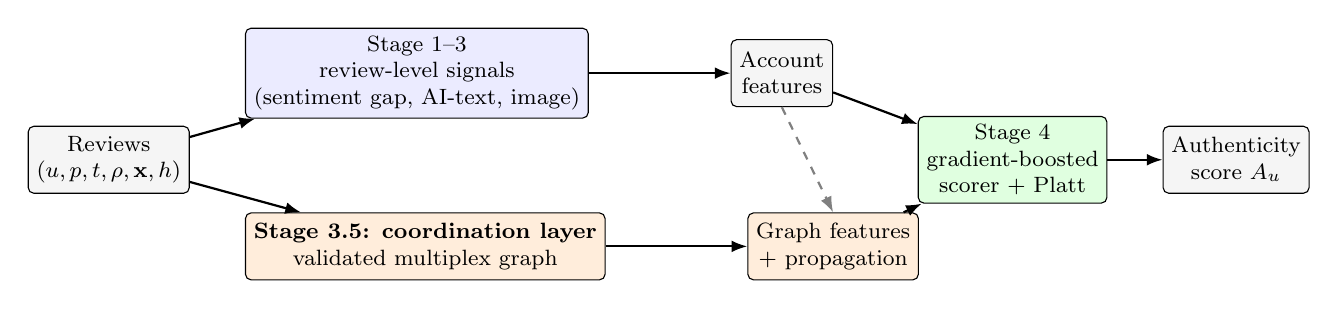
\begin{tikzpicture}[
  font=\footnotesize, node distance=5mm and 7mm,
  blk/.style={draw, rounded corners=2pt, align=center, minimum height=8.5mm, inner sep=3pt, fill=#1},
  blk/.default=gray!8, arr/.style={-{Latex[length=2mm]}, thick}]
\node[blk] (rev) {Reviews\\$(u,p,t,\rho,\mathbf x,h)$};
\node[blk=blue!8, right=of rev, yshift=11mm] (s1) {Stage 1--3\\review-level signals\\(sentiment gap, AI-text, image)};
\node[blk=orange!14, right=of rev, yshift=-11mm] (g) {\textbf{Stage 3.5: coordination layer}\\validated multiplex graph};
\node[blk, right=18mm of s1] (acc) {Account\\features};
\node[blk=orange!14, right=18mm of g] (gf) {Graph features\\+ propagation};
\node[blk=green!12, right=14mm of $(acc)!0.5!(gf)$] (st4) {Stage 4\\gradient-boosted\\scorer + Platt};
\node[blk, right=7mm of st4] (out) {Authenticity\\score $A_u$};
\draw[arr] (rev) -- (s1); \draw[arr] (rev) -- (g);
\draw[arr] (s1) -- (acc); \draw[arr] (g) -- (gf);
\draw[arr] (acc) -- (st4); \draw[arr] (gf) -- (st4); \draw[arr] (st4) -- (out);
\draw[arr, dashed, gray] (acc.south) -- (gf.north);
\end{tikzpicture}}
\caption{Pipeline. Stages 1--3 produce review-level signals (sentiment gap, AI-text score, image--text mismatch). The coordination layer (orange) is the contribution of this paper; the dashed arrow shows the out-of-fold base score used only for propagation.}\label{fig:arch}
\end{figure}

\subsection{Three evidence layers}\label{sec:layers}

Each layer yields, for pairs of accounts $(u,v)$, an observed count $k^{(\ell)}_{uv}$ of coordination-like coincidences, together with a null expectation $\mu^{(\ell)}_{uv}$ that accounts for how active and how ``popular'' the accounts and the shared items are.

\paragraph{Sync layer (co-review synchrony).} Let an \emph{event} be a product--week pair $e=(p,\lfloor t/W\rfloor)$ with $W=7$ days. Let $B_{ue}=1$ if $u$ reviewed in $e$, $n_u=\sum_eB_{ue}$, $s_e=\sum_uB_{ue}$ and $S=\sum_es_e$. The observed count is $k_{uv}=\sum_eB_{ue}B_{ve}$. Under a bipartite Chung--Lu null in which $u$ attends $e$ independently with probability $\pi_{ue}=n_us_e/S$,
\begin{equation}\label{eq:mu}
\mu_{uv}=\sum_e\pi_{ue}\pi_{ve}=\frac{n_un_v}{S^{2}}\sum_e s_e^{2}.
\end{equation}
The sum $\sum_es_e^2$ is large when a few events (sale weeks, blockbuster products) concentrate many reviews, which raises $\mu_{uv}$ and prevents hubs from generating significance by themselves.

\paragraph{Content layer (near-duplicate text).} Review $i$ is a near-duplicate of $j$ if $\cos(\mathbf x_i,\mathbf x_j)\ge\theta$ ($\theta=0.8$) and the authors differ. Let $\deg_i$ be the number of such neighbours, $D_u=\sum_{i\in\mathcal R_u}\deg_i$, and let $k_{uv}$ count near-duplicate pairs between $u$ and $v$. A degree-corrected null on the review-similarity graph gives $\mu_{uv}=D_uD_v/\sum_i\deg_i$. Accounts that write generic phrases have large $D_u$, so they need many more matches than a pair of accounts that rarely resemble anyone---this is the \emph{genericness correction}. For real review text, we replace dense embeddings by hashed word 4-gram shingles with exact sparse cosine similarity (Section~\ref{sec:real_design}); the null is unchanged.

\paragraph{Media layer (shared images).} With $g_h$ the number of accounts that used fingerprint $h$, $k_{uv}$ counts fingerprints shared by $u$ and $v$ and $D_u=\sum_{h\in u}(g_h-1)$, giving $\mu_{uv}=D_uD_v/\sum_wD_w$, so catalogue photographs used by many buyers carry little weight.

\subsection{Validation and fusion}

For each layer, pairs with $k_{uv}\ge k_{\min}$ are tested ($k_{\min}=2$ for all layers in the headline results; $k_{\min}=1$ for shingle-based content on real text is an exploratory setting that the label-free rule of Section~\ref{sec:real_design} rejects) against the one-sided Poisson tail
\begin{equation}\label{eq:p}
p_{uv}=\Pr\{\mathrm{Poisson}(\mu_{uv})\ge k_{uv}\},
\end{equation}
where the number of hypotheses is the number of pairs with at least one coincidence (the testable pairs, as in statistically validated networks \citep{tumminello2011}). Edges are kept by the Benjamini--Hochberg procedure at level $q=0.01$ \citep{benjamini1995}, and an edge confidence $a^{(\ell)}_{uv}=\min\{1,-\log_{10}p_{uv}/10\}$ is assigned. Layers are fused by noisy-OR,
\begin{equation}\label{eq:nor}
a_{uv}=1-\prod_{\ell}\bigl(1-a^{(\ell)}_{uv}\bigr),
\end{equation}
which is monotone, never lower than the strongest layer, and treats a missing layer as neutral; edges with $a_{uv}\ge0.3$ form the weighted graph $\mathbf W$.

\begin{proposition}[Quality of the Poisson tail]\label{prop:poisson}
Under the Chung--Lu null with $\pi_{ue}\pi_{ve}\le 1$, the count $K_{uv}$ is a sum of independent Bernoulli variables with success probabilities $\pi_{ue}\pi_{ve}$, and its total-variation distance to $\mathrm{Poisson}(\mu_{uv})$ is at most $\sum_e(\pi_{ue}\pi_{ve})^2\le\mu_{uv}\max_e\pi_{ue}\pi_{ve}$.
\end{proposition}
\begin{proof}
The first statement is the definition of the null. The bound is Le Cam's inequality for sums of independent Bernoulli variables.
\end{proof}
The p-values of different pairs share accounts and are therefore dependent, so Benjamini--Hochberg control is not guaranteed by the usual independence argument; we therefore check calibration empirically on a null market (Section~\ref{sec:results}).

\subsection{Account features, communities and propagation}

\paragraph{Graph features.} For each account: weighted degree (strength) and degree, per-layer strengths, number of layers touching the account, the unweighted clustering coefficient, the $k$-core number, and the strength and degree restricted to \emph{multi-layer edges} (edges present in at least two layers). Communities are found by Louvain modularity optimisation \citep{blondel2008} (resolution 1, seeded), which is fast but subject to the resolution limit \citep{fortunato2007}; a well-connectedness-preserving alternative exists \citep{traag2019}. Each community yields size, internal density, \emph{focus} (share of its reviews on its three most-reviewed products), a Herfindahl concentration of its product shares, and \emph{temporal compactness} (one minus ten times the inter-quartile range of review times on its top product, relative to the observation horizon, truncated to $[0,1]$). These describe what a campaign cell looks like---few targets, tight timing---without using any label.

\paragraph{Propagation.} Let $s^0_u$ be an out-of-fold probability from a gradient-boosted classifier trained on the review-level and metadata features only, $\mathbf P$ the row-normalised $\mathbf W$ (isolated accounts receive a self-loop), and $\alpha=0.8$. Suspicion is spread by
\begin{equation}\label{eq:prop}
\mathbf s=(1-\alpha)\,\mathbf s^0+\alpha\,\mathbf P\,\mathbf s,\qquad\text{so}\qquad \mathbf s=(1-\alpha)(\mathbf I-\alpha\mathbf P)^{-1}\mathbf s^0 .
\end{equation}
This is the stationary form of a random walk with restart, as used in graph-based semi-supervised learning \citep{zhou2004}, but seeded with a calibrated, label-free-at-test-time base score rather than with known labels.

\begin{proposition}[Well-posedness of propagation]\label{prop:prop}
For $\alpha\in[0,1)$ and row-stochastic $\mathbf P$, Eq.~\eqref{eq:prop} has a unique solution, the iteration $\mathbf s^{m+1}=(1-\alpha)\mathbf s^0+\alpha\mathbf P\mathbf s^{m}$ converges to it geometrically at rate $\alpha$, and every $s_u$ is a convex combination of the entries of $\mathbf s^0$; in particular $\min\mathbf s^0\le s_u\le\max\mathbf s^0$.
\end{proposition}
\begin{proof}
$\|\alpha\mathbf P\|_\infty=\alpha<1$, so $\mathbf I-\alpha\mathbf P$ is invertible and $(\mathbf I-\alpha\mathbf P)^{-1}=\sum_{m\ge0}\alpha^m\mathbf P^m$ (Neumann series), which gives uniqueness and the rate $\alpha$. Each $\mathbf P^m$ is row-stochastic, and $(1-\alpha)\sum_m\alpha^m=1$, so every row of $(1-\alpha)(\mathbf I-\alpha\mathbf P)^{-1}$ is a probability vector.
\end{proof}

\subsection{Stage-4 scorer and calibration}
The final scorer is an XGBoost classifier \citep{chen2016} on $[\,$review-level features, metadata, graph features, propagated score, neighbour-mean of $s^0\,]$ (150 trees, depth 3, learning rate 0.08, subsample 0.8, column subsample 0.8, $L_2$ 2.0). Probabilities are calibrated by Platt scaling \citep{platt1999} on a validation fold, the operating threshold maximises $F_1$ on that fold, and the authenticity score is $A_u=100(1-\hat p_u)$.

\paragraph{Complexity.} The sync layer costs the sparse product $\mathbf B\mathbf B^{\top}$, i.e.\ $O(\sum_es_e^2)$; the media layer $O(\sum_hg_h^2)$; the content layer is implemented as exact chunked cosine search, $O(N^2d)$ for $N$ reviews, which an approximate nearest-neighbour index would reduce; Louvain is close to linear in the number of edges. Measured scaling is reported in Section~\ref{sec:results}.

\section{Controlled Simulation Design}\label{sec:design}

\subsection{What is simulated, and why}\label{sec:why}
The simulation below is a secondary, controlled stress test; the primary evidence is Section~\ref{sec:real_design}. 
Reviews from real Indian marketplaces with ground-truth labels of paid campaigns are not publicly available, and a platform's internal moderation logs are not accessible to outside researchers. Evaluating a coordination detector on scraped data would therefore have no reliable labels, while a simulation offers known ground truth, controlled adversaries and repeatable seeds. The price is external validity: findings hold for the generative assumptions made. We therefore (i) document every assumption (Table~\ref{tab:sim}), (ii) sweep the assumptions that matter most (upstream detector quality, prevalence, observability), (iii) include honest behaviours designed to \emph{confuse} the method, and (iv) provide the real-data protocol of Appendix~\ref{app:real}.

\subsection{CampaignSim}
Every market realisation is generated from a seed; Table~\ref{tab:sim} gives the default configuration.

\begin{table}[t]
\caption{CampaignSim default configuration (baseline scenario). ``Honest'' parameters describe genuine behaviour; ``campaign'' parameters describe paid cells.}\label{tab:sim}
\small
\begin{tabular}{@{}p{2.8cm}p{8.4cm}@{}}
\toprule
Component & Specification \\
\midrule
Market & 4{,}000 honest accounts, 250 products in 15 categories, 365 days; six languages (hi, ta, te, bn, mr, gu) with shares .30/.18/.14/.14/.12/.12 \\
Honest activity & $1+\mathrm{NB}(2,0.4)$ reviews per account (mean 3); product choice from Zipf popularity (exponent 1.0), 70\% within two favourite categories; times follow product launch plus an exponential tail (mean 60 d), and 35\% of reviews fall into four 7-day sale windows \\
Honest hard negatives & 30\% \emph{terse} writers (generic phrases, 6 per language, near-identical embeddings); 5\% of honest reviews \emph{LLM-assisted}; 4\% of accounts in households of 3--6 who review 2--4 products together; 5\% of products with a flash-sale crowd of 15--40 honest reviewers within about a day; 3\% of image-bearing honest reviews reuse the product's catalogue photo \\
Text embeddings & $d=24$; honest: category + language topic plus noise; campaign: unit template vector plus paraphrase noise of scale $\sigma$ (default 0.6; two templates per cell), so within-template cosine is about $1/(1+\sigma^2)$ \\
Campaigns & fake accounts $=8\%$ of all accounts; cells of 6--18 workers; 3--6 target products (chosen with a bias to less popular products); each worker reviews a target with probability 0.7; burst spread: exponential, mean 3 days; 25\% of bursts placed inside sale windows; 30\% of campaigns attack a competitor (1--2 stars), the rest boost (4--5 stars); camouflage: every worker is padded with honest-looking reviews up to an honest activity level ($1+\mathrm{NB}(2,0.4)$ reviews in total), so that review counts do not give workers away; 50\% of campaign reviews carry an image, drawn from a pool of 6 per cell with prob.\ 0.7; 30\% of workers use freshly created accounts, the rest aged accounts; 60\% of campaign reviews are LLM-written \\
Upstream signals & $s_{\mathrm{txt}}\sim\mathcal N(\mu_{\ell}\mathbb 1[\text{LLM-written}],1)$ with $\mu_\ell=\sqrt2\,\Phi^{-1}(\mathrm{AUC}_\ell)$ and AUC per language .92/.85/.83/.88/.85/.82 (hi/ta/te/bn/mr/gu); image mismatch score with AUC .85; sentiment-gap magnitude slightly larger for campaign reviews \\
\bottomrule
\end{tabular}
\end{table}

The upstream detector scores are \emph{modelled}, not computed from text: the aim is to ask how much a coordination layer adds when review-level detectors have a stated, adjustable quality. The per-language AUCs are assumptions, set to a plausible-to-pessimistic range and swept from 0.55 to 0.95 in Section~\ref{sec:results}; they are not measurements of the earlier MultiSentinel modules. Note that an AI-text score is evidence of LLM \emph{use}, not of fraud: honest AI-assisted writers receive high scores and campaign reviews written by humans do not.

\subsection{Adversary scenarios}
Table~\ref{tab:scen_def} lists the nine scenarios. Each changes only the stated parameters of the baseline.

\begin{table}[t]
\caption{Scenarios. Only the listed parameters differ from the baseline in Table~\ref{tab:sim}.}\label{tab:scen_def}
\small
\begin{tabular}{@{}p{3.0cm}p{8.4cm}@{}}
\toprule
Scenario & Change \\
\midrule
S0 Baseline & none \\
S1 Paraphrase evasion & paraphrase noise $\sigma=1.0$ (near-duplicate cosine about 0.5); AI-text detector separation on campaign reviews halved \\
S2 Temporal jitter & burst spread 30 days; no sale-window placement \\
S3 Cell fragmentation & cells of 3--6 workers, 2--4 targets \\
S4 Heavy camouflage & two extra camouflage reviews per worker, placed on the 20 most popular products inside sale windows (maximising accidental overlap with honest users) \\
S5 Image diversification & no image reuse; image-mismatch AUC 0.70 \\
S6 Sale-window blending & every burst placed inside a sale window \\
S7 Adaptive (combined) & $\sigma=1.0$, halved AI-text separation, 20-day spread, hub-and-sale camouflage as in S4, image reuse 0.1, cells of 4--10, 60\% of bursts in sale windows \\
S8 Dense honest crowds & 60\% of honest reviews in sale windows, flash crowds on 15\% of products, households 8\% of accounts \\
\bottomrule
\end{tabular}
\end{table}

\subsection{Evaluation protocol}
\paragraph{Splits and leakage control.} Accounts are assigned to five folds \emph{by group}: every campaign cell and every honest household is one group, and fake and honest groups are spread evenly over folds. For fold $k$, fold $k$ is the test set, fold $k+1$ the validation set (used for Platt scaling and for choosing the operating threshold) and the rest the training set. The coordination graph and its features are built without labels. The propagation seed $s^0$ is computed afresh in every outer fold: out-of-fold inside the training and validation accounts, and from a model fitted on them for the test accounts, so no test label reaches any feature. Pooled out-of-fold predictions from the five folds form one evaluation per market realisation.

\paragraph{Metrics.} Average precision (AP, the primary metric because campaign accounts are a minority \citep{saito2015}), AUROC, $F_1$ at the validation-chosen threshold, recall at 1\% false-positive rate, and expected calibration error \citep{guo2017,niculescu2005} with ten bins. Campaign recovery is the share of campaign cells that have a detected community with Jaccard overlap $\ge0.5$. We also report false-positive rates on honest sub-populations.

\paragraph{Replication and statistics.} Each scenario is run on independent market realisations (15 for the baseline, 10 for each other scenario, 4 per sweep point). We report means with 95\% $t$-intervals over realisations, paired differences against the graph-free scorer with a bootstrap interval, the exact paired Wilcoxon signed-rank test, and Holm correction over scenarios. \emph{Design history, disclosed for transparency.} Hyper-parameters (window, similarity threshold, propagation weight, model settings) were fixed a priori; seed 1000 was used for debugging and is not part of any reported run. Two changes were made after inspecting earlier complete runs, both because of validity problems rather than accuracy tuning: (i) the camouflage model was corrected, since the first version added reviews to campaign accounts and thereby made them easier to catch by activity level alone; (ii) the validation level was tightened to $q=0.01$ and a minimum of two coincidences was required for the content layer, after the null-calibration experiment (Section~\ref{sec:res_null}) showed that the content layer was not calibrated. Each correction led to a complete re-run; only runs of the final code are reported, and the number of replicates per scenario was raised to 10 so that the paired test can survive Holm correction. One planned baseline realisation was excluded for a non-terminating routine (Section~\ref{sec:results}).

\subsection{Baselines}
\begin{itemize}
\item \emph{Single-signal scorers}: AI-text detector only; image check only; reviewer metadata only (gradient boosting on aggregates).
\item \emph{Stage-fusion}: the original MultiSentinel Stage~4 design, i.e.\ review-level signals plus metadata, with no graph.
\item \emph{Raw co-review graph with neighbour aggregation}: the same features plus one- and two-hop neighbour means taken over an \emph{unvalidated} co-review graph (accounts sharing at least two product--week events); this is a strong, learning-free analogue of graph-neural aggregation.
\item \emph{Dense-block peeling} (unsupervised): greedy peeling of the account--event bipartite graph with column down-weighting, in the spirit of \citet{hooi2016}; our implementation is a simplified re-implementation, not the authors' code.
\item \emph{Graph features only}: no review-level signals, to separate the contribution of structure.
\end{itemize}
On YelpZip we also include a trained GraphSAGE network and a no-graph control (Section~\ref{sec:real_design}); trained graph networks were not run in the simulation or injection experiments (Section~\ref{sec:limits}). In every experiment of this paper the review-level signals are modelled (simulation) or computed with a TF-IDF classifier (Yelp); the trained mBERT, RoBERTa and CLIP modules are not run.

\section{Real-Data Evaluation Design}\label{sec:real_design}

\paragraph{Data and labels.} YelpZip \citep{rayana2015} contains \num{yz_nrev} reviews by \num{yz_nacc} reviewers of restaurants and hotels in the New York area, each with a rating, a date and the text. The label of a review is whether Yelp's production filter placed it in the ``not recommended'' list (\num{yz_prev}\% of reviews). This is a platform decision, not verified fraud: the filter is believed to use behavioural and textual signals, so our target is partly the filter's own logic, and some filtered reviews are genuine. All statements below about ``fraud'' or ``spam'' should be read as ``filtered by Yelp''. The corpus has no image data and no account-creation date, so the media layer is empty and the metadata features are derived from the review history. The data were obtained from the corpus authors' release and are not redistributed.

\paragraph{Review-level signals.} The AI-text score $s_{\mathrm{txt}}$ of the earlier MultiSentinel modules is not meaningful for 2010s English text. We replace it by an out-of-fold score from a TF-IDF logistic regression on review text, computed with reviewer-grouped folds, so that no review is scored by a model that saw its author. The rating--sentiment gap and image signals are not used. The ``text only'' row of Table~\ref{tab:yelp} is this score alone.

\paragraph{Layers.} The \emph{sync} layer uses product--week events as in Section~\ref{sec:layers} (\num{yz_e_sync} validated edges). For the \emph{content} layer on real text we use hashed word 4-gram shingles (binary, $2^{24}$ features, document-frequency filter 2--200, at least five informative 4-grams per review) and exact sparse cosine similarity with $\theta=0.6$ between reviews of different accounts. A first attempt with a dense low-rank projection of TF-IDF found only 33 near-duplicate pairs and was discarded. Shingle near-duplicates are plausible without using any label: 93\% of near-duplicate pairs concern the same restaurant, against 0.14\% for random pairs. \emph{Choice of $k_{\min}$ and what it revealed.} With $k_{\min}=2$ the content layer yields only \num{yz_e_c2} edges; with $k_{\min}=1$ it yields \num{yz_e_c1}. We first used $k_{\min}=1$ after seeing that $k_{\min}=2$ left the layer almost empty and that content edges were enriched for filtered reviews, which was not label-blind. We therefore fixed a label-free rule afterwards and apply it to the headline result: permute the authorship of reviews (globally, and within product) so that real near-duplicate texts remain but account links are destroyed, and take the smallest $k_{\min}$ for which at most one content edge survives validation at $q=0.01$ on every permutation. At $k_{\min}=1$ the permuted data yield about \num{yz_perm1} validated edges (all of the \num{yz_ntest} candidate pairs have a tiny expected count under the degree-corrected null, so a single coincidence is `significant'), against \num{yz_e_c1} on the real data; at $k_{\min}=2$ no permutation yields an edge (maximum \num{yz_perm2}). The rule selects $k_{\min}=2$, which is the proposed setting in all YelpZip results; the $k_{\min}=1$ configuration is reported as an exploratory variant and should be read as a near-duplicate graph without effective statistical control.

\paragraph{Protocol.} Evaluation is at the review level. Reviewers are assigned to five folds with \texttt{StratifiedGroupKFold} (all reviews of a reviewer in one fold); predictions are pooled out-of-fold; the graph is built without labels; the propagation seed $s^0$ is recomputed per outer fold from inner out-of-fold scores; the model is XGBoost (150 trees, depth 3, learning rate 0.08) with Platt scaling on a validation fold. Three seeds (fold assignments and model randomness) are run. Uncertainty for paired differences is a cluster bootstrap over reviewers.

\paragraph{Baselines.} Besides those of Section~\ref{sec:design}, we add \emph{account context}: stage-fusion plus the mean out-of-fold base score of the reviewer's other reviews and review count, with no graph. This baseline isolates the part of the apparent graph gain that comes from pooling a reviewer's own evidence rather than from coordination.

\paragraph{Trained GNN baseline.} We add a two-layer GraphSAGE network (mean aggregator, 64 hidden units, Adam, 120 epochs, implemented in PyTorch) on the \emph{unvalidated} union of raw co-review and raw near-duplicate pairs. Node inputs are standardised account-level means of the review features, the account's out-of-fold base score and log review count. The network is trained on account nodes of the training and validation folds with soft targets (share of filtered reviews, weighted by review count); its logit is added as one feature to the account-context model. To avoid leakage, logits for training accounts come from five inner masked-label runs, and logits for test accounts from a network trained on all training and validation accounts. A control is the same network with an empty graph (a neural account model), which separates the contribution of graph edges from that of a non-linear account model.

\paragraph{Injected campaigns.} To obtain known ground truth on a real background, we keep only reviewers with no filtered review (\num{inj_bg} accounts, taken as the genuine background; the assumption is that Yelp's filter is high-recall for them, which we cannot verify) and inject $4\%$ additional accounts organised in cells. Campaign texts are sampled from real filtered reviews (not generated by an LLM), cells review 2--6 targets within a time window, and each account is padded with honest-looking reviews cloned from background donors so that activity level alone is not a giveaway. Six scenarios vary the adversary: I0 baseline (7-day window, light text edits); I1 paraphrase (35\% word drops, 25\% replacements); I2 temporal jitter (60-day window); I3 fragmentation (cells of 3--6); I4 camouflage (reviews on popular hub venues); I5 adaptive (all of the above combined). Evaluation is at the account level. Even in I0 a metadata-only scorer reaches an AP of about 0.64, so the injection is not trivially separable; we did not tune it to make the problem harder after seeing this. Results are over three seeds per scenario. The text scores of background and campaign reviews are drawn from the reviewer-grouped out-of-fold TF-IDF score of YelpZip, as a modelled detector in the sense of the simulation. The evaluation target is injected versus genuine, which is unrelated to Yelp's filter labels, so no label of an evaluated account reaches a feature, and we did not recompute these scores inside outer folds.

\section{Results on Real Data}\label{sec:real_results}

\subsection{YelpZip}\label{sec:res_yelp}
\paragraph{Protocol correction.} Our first YelpZip runs used a text score computed once by out-of-fold logistic regression with its own reviewer folds, which let labels of reviewers in an outer test fold influence the text feature of training reviews. We therefore recomputed the text score \emph{inside} every outer fold (inner reviewer-grouped out-of-fold on the training and validation reviewers, one model on all of them for the test reviewers). This lowers every absolute number by about 0.01 AP. All YelpZip and YelpNYC results reported in this paper, including the additional baselines (Table~\ref{tab:yelp_old}), the ablations (Table~\ref{tab:yelp_abl}) and the sensitivity sweeps (Table~\ref{tab:sens}), use the corrected protocol with three seeds. The injection experiments do not use Yelp labels as their target (Section~\ref{sec:res_inject}).

\paragraph{Main comparison.} The proposed scorer (rule-selected $k_{\min}=2$) reaches AP \num{yz_ap_full} against \num{yz_ap_stage} for stage-fusion without a graph, a paired difference of \num{yz_d_stage} AP (95\% cluster-bootstrap CI \num{yz_d_stage_lo}--\num{yz_d_stage_hi}, seed-0 pooled predictions). That is a small improvement over review-level signals.

\begin{table}[t]
\caption{YelpZip, review level, text score recomputed inside each outer fold, pooled out-of-fold. AP is mean $\pm$ SD over three seeds. Label: Yelp filter decision (prevalence \num{yz_prev}\%).}\label{tab:yelp}
\small\setlength{\tabcolsep}{3pt}
\begin{tabular}{@{}lcccc@{}}
\toprule
Method & AUROC & AP & $F_1$ & Rec@1\%FPR \\
\midrule
Text only (TF-IDF LR) & 0.725 & 0.293 $\pm$ 0.001 & 0.357 & 0.059 \\
Stage-fusion (text + behaviour) & 0.854 & 0.465 $\pm$ 0.001 & 0.487 & 0.125 \\
Stage-fusion + account context (no graph) & 0.861 & 0.478 $\pm$ 0.000 & 0.497 & 0.130 \\
MultiSentinel-G (proposed, $k_{\min}=2$) & 0.862 & 0.478 $\pm$ 0.002 & 0.498 & 0.131 \\
Neural account model, no graph (MLP) & 0.865 & 0.482 $\pm$ 0.002 & 0.501 & 0.134 \\
GraphSAGE (trained GNN) & 0.867 & 0.491 $\pm$ 0.003 & 0.504 & 0.140 \\
\bottomrule
\end{tabular}
\end{table}

\paragraph{Most of the gain is reviewer context, not coordination.} Adding the reviewer's own aggregated base scores, without any graph, already lifts AP to \num{yz_ap_ctx} (0.013 over stage-fusion). Against this stronger baseline the increment of the coordination graph is \num{yz_d_ctx_mean} AP on average over seeds and \num{yz_d_ctx} AP (bootstrap CI \num{yz_d_ctx_lo}--\num{yz_d_ctx_hi}) in the seed-0 pooled predictions, so at most a very small contribution; in one of three seeds the proposed scorer is below account context. The learning-free raw co-review aggregation is practically level with the proposed scorer (AP \num{yz_ap_raw} against \num{yz_ap_full}; Table~\ref{tab:yelp_old}), and graph features alone are weak (AUROC 0.562). The unsupervised dense-block baseline is \emph{inverted} (AUROC \num{yz_auc_dense}), i.e.\ filtered reviews sit in less dense regions than genuine ones, consistent with Yelp-filtered reviews being sparse, isolated posts.

\paragraph{Trained neural baselines are better.} A GraphSAGE network (description above) reaches AP \num{yz_ap_gnn} and AUROC \num{yz_auc_gnn} (mean of three seeds). The paired differences and bootstrap intervals below use the seed-0 predictions (GNN AP \num{yz0_ap_gnn}, MLP \num{yz0_ap_mlp}): the GNN is \num{yz_d_gnnfull} AP above the proposed scorer (CI \num{yz_d_gnnfull_lo}--\num{yz_d_gnnfull_hi}). The same network without graph edges is \num{yz_d_mlpfull} above the proposed scorer (CI \num{yz_d_mlpfull_lo} to \num{yz_d_mlpfull_hi}), and graph edges add \num{yz_d_gnnmlp} AP to the network (CI \num{yz_d_gnnmlp_lo}--\num{yz_d_gnnmlp_hi}). Two readings follow. First, a non-linear account-level model recovers at least as much as our validated layer on this corpus. Second, graph edges do help a trained network by a larger margin than they help ours, which suggests that a learned message-passing model uses the relational information more effectively than our hand-built features. The GNN is a black box on an unvalidated graph; the layer's practical advantages are statistically controlled, inspectable edges and campaign communities rather than higher accuracy on this benchmark.

\paragraph{Validated edges alone lose the benefit of the graph.} To test whether the statistical validation or the graph itself is responsible for the GNN's advantage, we trained the same network on (i) only our validated edges, weighted by confidence, and (ii) the unvalidated union plus our validated edges at full weight. In a single seed (seed 0), with only validated edges the network reaches AP \num{hyb_ap_val}, which is \num{hyb_d_valmlp} above the no-graph network (CI \num{hyb_d_valmlp_lo} to \num{hyb_d_valmlp_hi}), i.e.\ no detectable benefit, and \num{hyb_d_valgnn} (CI \num{hyb_d_valgnn_lo} to \num{hyb_d_valgnn_hi}) relative to the unvalidated-graph network. Adding validated edges to the unvalidated graph reaches \num{hyb_ap_mix}, \num{hyb_d_mixgnn} relative to the unvalidated graph alone (CI \num{hyb_d_mixgnn_lo} to \num{hyb_d_mixgnn_hi}), so validated edges do not add either. Error control on individual pairs removes edges that are insignificant one by one but informative together, and a learned model can exploit that.

\begin{table}[t]
\caption{YelpZip, corrected protocol (text score recomputed inside each outer fold), all baselines; mean over three seeds. The proposed row is $k_{\min}=2$; the last row is the exploratory $k_{\min}=1$ variant.}\label{tab:yelp_old}
\small\setlength{\tabcolsep}{3pt}
\begin{tabular}{@{}lcccc@{}}
\toprule
Method & AUROC & AP & $F_1$ & Rec@1\%FPR \\
\midrule
Text only (TF-IDF LR) & 0.725 & 0.293 & 0.357 & 0.059 \\
Behavioural only & 0.844 & 0.436 & 0.469 & 0.109 \\
Stage-fusion (text + behaviour) & 0.854 & 0.465 & 0.487 & 0.125 \\
Stage-fusion + account context (no graph) & 0.861 & 0.478 & 0.497 & 0.130 \\
Raw co-review graph + aggregation & 0.862 & 0.479 & 0.498 & 0.132 \\
Dense-block peeling & 0.281 & 0.106 & 0.063 & 0.000 \\
Graph features only & 0.562 & 0.161 & 0.254 & 0.028 \\
Neural account model, no graph (MLP) & 0.865 & 0.482 & 0.501 & 0.134 \\
GraphSAGE (trained GNN) & 0.867 & 0.491 & 0.504 & 0.140 \\
MultiSentinel-G (proposed, rule-selected $k_{\min}=2$) & 0.862 & 0.478 & 0.498 & 0.131 \\
Exploratory variant: content layer with $k_{\min}=1$ & 0.864 & 0.485 & 0.502 & 0.136 \\
\bottomrule
\end{tabular}
\end{table}

\paragraph{Where the graph applies.} Validated edges touch \num{yz_covacc}\% of reviewers (\num{yz_covacc_n}) and \num{yz_covrev}\% of reviews (seed-0 predictions). On these covered reviews AP is \num{yz_apcov_stage} for stage-fusion, \num{yz_apcov_ctx} with account context and \num{yz_apcov_full} with the graph; on the remaining reviews AP is \num{yz_apunc_ctx} with account context versus \num{yz_apunc_full}. The proposed graph therefore adds little even where it has coverage (about 0.004 AP over the context baseline), while the exploratory $k_{\min}=1$ variant reaches \num{yz_apcov_k1} against \num{yz_apcov_ctx_k1} for account context on \num{yz_covrev_k1}\% of reviews; since that setting was chosen after seeing labels and its validation is vacuous on real text (Section~\ref{sec:real_design}), we do not treat this larger covered-subset gain as evidence for coordination. The graph cannot help on reviews without edges.

\begin{table}[t]
\caption{YelpZip ablations (mean over three seeds). $\Delta$AP is relative to the exploratory $k_{\min}=1$ configuration (first row).}\label{tab:yelp_abl}
\small\setlength{\tabcolsep}{2pt}
\begin{tabular}{@{}lccc@{}}
\toprule
Variant & AP & AUROC & $\Delta$AP \\
\midrule
Exploratory $k_{\min}=1$ configuration (base of the ablations below) & 0.4846 & 0.8645 & +0.0000 \\
Proposed, rule-selected $k_{\min}=2$ & 0.4781 & 0.8617 & -0.0065 \\
Without sync layer & 0.4841 & 0.8647 & -0.0005 \\
Without content layer & 0.4782 & 0.8617 & -0.0064 \\
Without statistical validation & 0.4866 & 0.8650 & +0.0020 \\
Without propagation & 0.4845 & 0.8644 & -0.0001 \\
Without community features & 0.4839 & 0.8645 & -0.0007 \\
\bottomrule
\end{tabular}
\end{table}

\paragraph{Ablations.} The ablations are relative to the exploratory $k_{\min}=1$ configuration (corrected protocol, three seeds). No single component changes AP by more than about 0.007 (Table~\ref{tab:yelp_abl}); removing the sync layer leaves AP essentially unchanged even though coverage falls from 7{,}020 to 990 accounts (the pooled metric is dominated by uncovered reviews, so it is insensitive to which covered accounts are kept), and relaxing statistical validation slightly \emph{raises} AP, as in the simulation. These differences are of the order of the seed variation for several variants, so we do not rank the components; the ablation shows only that the effect is not carried by one layer.

\subsection{The account-context control on published-style graph methods}\label{sec:res_ctrl}
To test whether the control matters beyond our own method, we implemented two common ways of adding a graph to a review-level scorer and ran each with and without the account-context baseline as the reference. \emph{Propagation} spreads the out-of-fold base score over the graph (label-propagation style, as in our own propagation step). \emph{Neighbour aggregation} adds one- and two-hop neighbour means of account-level scores and the degree to the feature set of a gradient-boosted model (SIGN style). Both use the unvalidated co-review graph (``sync'') or the union of co-review and near-duplicate edges (``union''). These are our implementations of the methods' principle, not the original authors' code. Without the control the gain is measured against stage-fusion; with it, against stage-fusion plus account context (AP difference, three seeds; account context alone adds \num{ctrl_ctxgain}).

\begin{table}[t]
\caption{Apparent and control-adjusted AP gain of graph additions on YelpZip (corrected protocol, mean of three seeds). ``Without control'': versus stage-fusion; ``with control'': versus stage-fusion plus account context; the last column is the share of the apparent gain that disappears under the control.}\label{tab:ctrl}
\footnotesize\setlength{\tabcolsep}{3pt}
\begin{tabular}{@{}llccc@{}}
\toprule
Graph addition & Graph & Without control & With control & Share lost \\
\midrule
Propagation (LP style) & sync & +0.0095 & +0.0003 & 97\% \\
Propagation (LP style) & union & +0.0096 & +0.0007 & 92\% \\
Aggregation (SIGN style) & sync & +0.0017 & +0.0012 & 27\% \\
Aggregation (SIGN style) & union & +0.0071 & +0.0053 & 25\% \\
\bottomrule
\end{tabular}
\end{table}

For propagation the control removes almost the entire gain (\num{ctrl_lp_sync_share}\% on the co-review graph and \num{ctrl_lp_union_share}\% on the union graph): what looks like a graph effect of about \num{ctrl_lp_sync_no} AP is, to within seed variation, what pooling a reviewer's own scores already provides. For learned neighbour aggregation the effect is smaller (\num{ctrl_sign_union_share}\% lost on the union graph, \num{ctrl_sign_sync_share}\% on the co-review graph, where the gain is tiny to begin with), and a real, small relational contribution of about \num{ctrl_sign_union_with} AP remains. The control therefore does not make every graph gain disappear, and it should be reported, not assumed to erase it.

We repeated the comparison for the trained GraphSAGE network (three seeds). Its node features already contain reviewer-level aggregates, so it carries the account context itself. Giving the downstream scorer the context column or not changes the GNN's AP only from 0.4907 to 0.4911, and the no-graph MLP from 0.4827 to 0.4822. The GNN's edge over the MLP is about 0.008--0.009 AP in both cases. On YelpNYC the pattern is the same: GNN 0.4003 with and 0.3995 without the context column, MLP 0.3893 and 0.3878, an edge of about 0.011 AP. The control therefore removes the gain of propagation-style additions, but does not remove the small gain of a GNN that already sees reviewer-level features. We do not claim that this small gain is caused by coordination structure: the GNN also aggregates over unvalidated co-review edges, which friend groups and crowds populate (Section~\ref{sec:res_open}).

\subsection{Replication on YelpNYC}\label{sec:res_nyc}
We repeated the corrected protocol on the Kaggle release of YelpNYC (\num{nyc_nrev} reviews, \num{nyc_nacc} reviewers, \num{nyc_nprod} restaurants, \num{nyc_prev}\% filtered), obtained as two files whose rows we verified to agree on restaurant and date for every review. This is not independent data in the strict sense: it covers New York restaurants from the same platform and the same filter, and probably overlaps the restaurants in YelpZip; it shows that the pipeline and its conclusions do not hinge on one particular file or size. The label-free rule selects $k_{\min}=2$ again: authorship permutations yield about \num{nyc_perm1} validated content edges at $k_{\min}=1$ (against \num{nyc_e1} real) and none at $k_{\min}=2$ (\num{nyc_e2} real edges). The graph is even sparser than on YelpZip (\num{nyc_cov}\% of reviewers touched by a sync edge).

\begin{table}[t]
\caption{YelpNYC, review level, corrected protocol (text score recomputed inside each outer fold). AP is mean $\pm$ SD over three seeds.}\label{tab:nyc}
\small\setlength{\tabcolsep}{3pt}
\begin{tabular}{@{}lcccc@{}}
\toprule
Method & AUROC & AP & $F_1$ & Rec@1\%FPR \\
\midrule
Text only (TF-IDF LR) & 0.709 & 0.226 $\pm$ 0.001 & 0.295 & 0.055 \\
Stage-fusion (text + behaviour) & 0.837 & 0.365 $\pm$ 0.001 & 0.409 & 0.108 \\
Stage-fusion + account context (no graph) & 0.846 & 0.384 $\pm$ 0.001 & 0.421 & 0.120 \\
MultiSentinel-G (proposed, $k_{\min}=2$) & 0.846 & 0.386 $\pm$ 0.001 & 0.421 & 0.120 \\
Neural account model, no graph (MLP) & 0.849 & 0.389 $\pm$ 0.001 & 0.426 & 0.122 \\
GraphSAGE (trained GNN) & 0.852 & 0.400 $\pm$ 0.003 & 0.429 & 0.127 \\
\bottomrule
\end{tabular}
\end{table}

The pattern is the same as on YelpZip (Table~\ref{tab:nyc}). The proposed scorer improves on stage-fusion by \num{nyc_d_stage} AP (CI \num{nyc_d_stage_lo}--\num{nyc_d_stage_hi}), but its increment over account context is \num{nyc_d_ctx_mean} AP on average over seeds (\num{nyc_d_ctx}, CI \num{nyc_d_ctx_lo}--\num{nyc_d_ctx_hi}, seed 0), a borderline value. On seed 0, GraphSAGE is \num{nyc_d_gnnfull} AP above the proposed scorer (CI \num{nyc_d_gnnfull_lo}--\num{nyc_d_gnnfull_hi}), and the neural model without graph is \num{nyc_d_mlpfull} above it (CI \num{nyc_d_mlpfull_lo}--\num{nyc_d_mlpfull_hi}), which is statistically level. Graph edges add \num{nyc_d_gnnmlp} AP to the neural model (CI \num{nyc_d_gnnmlp_lo}--\num{nyc_d_gnnmlp_hi}). Injection and sensitivity experiments were not repeated on YelpNYC.

\subsection{Sensitivity to parameters}\label{sec:res_sens_real}
Table~\ref{tab:sens} varies the sync window (3, 7, 14, 30 days), the false-discovery level ($q=0.001$ to $0.05$, for both layers) and the propagation weight ($\alpha=0.5$ to $0.95$) one at a time, with the same folds and three seeds. Average precision stays between \num{sens_min} and \num{sens_max} in every setting, i.e.\ within about 0.002 of the proposed setting and less than 0.002 above the graph-free baseline (0.4778). The result is stable, but the flatness mostly reflects how little the graph contributes on this corpus. We did not vary the similarity threshold $\theta$ of the content layer, which would require rebuilding the pair list. Table~\ref{tab:injfrac} varies the share of injected accounts (1\%--8\%) for the baseline and temporal-jitter scenarios (one seed): the gain of the proposed scorer over stage-fusion is larger at low prevalence (about 0.33 at 1\% in I0) and shrinks as stage-fusion improves at 8\%, but remains positive, and the proposed scorer stays ahead of raw co-review aggregation in I0 and far ahead under jitter at every prevalence.

\begin{table}[t]
\caption{Parameter sensitivity on YelpZip (mean $\pm$ SD of AP over three seeds, AUROC mean). Settings are varied one at a time from the proposed setting.}\label{tab:sens}
\small\setlength{\tabcolsep}{3pt}
\begin{tabular}{@{}lcc@{}}
\toprule
Setting & AP & AUROC \\
\midrule
No graph (account context) & 0.4778 $\pm$ 0.0002 & 0.8612 \\
Proposed (7 days, $q=0.01$, $\alpha=0.8$) & 0.4781 $\pm$ 0.0019 & 0.8617 \\
Window 3 days & 0.4782 $\pm$ 0.0017 & 0.8615 \\
Window 14 days & 0.4795 $\pm$ 0.0010 & 0.8616 \\
Window 30 days & 0.4797 $\pm$ 0.0004 & 0.8615 \\
$q=0.001$ & 0.4787 $\pm$ 0.0019 & 0.8615 \\
$q=0.05$ & 0.4797 $\pm$ 0.0014 & 0.8617 \\
$\alpha=0.5$ & 0.4787 $\pm$ 0.0021 & 0.8618 \\
$\alpha=0.95$ & 0.4793 $\pm$ 0.0013 & 0.8617 \\
\bottomrule
\end{tabular}
\end{table}

\begin{table}[t]
\caption{Injected-campaign prevalence sweep (account-level AP, seed 0). $\Delta$: proposed minus stage-fusion.}\label{tab:injfrac}
\small\setlength{\tabcolsep}{3pt}
\begin{tabular}{@{}llcccc@{}}
\toprule
Scenario & Injected & Stage-fus. & Raw graph & Proposed & $\Delta$ \\
\midrule
I0 & 1\% & 0.500 & 0.727 & 0.833 & 0.332 \\
I0 & 2\% & 0.601 & 0.776 & 0.861 & 0.260 \\
I0 & 4\% & 0.697 & 0.818 & 0.887 & 0.191 \\
I0 & 8\% & 0.781 & 0.861 & 0.912 & 0.131 \\
I2 & 1\% & 0.456 & 0.476 & 0.740 & 0.283 \\
I2 & 2\% & 0.551 & 0.567 & 0.788 & 0.237 \\
I2 & 4\% & 0.654 & 0.667 & 0.833 & 0.179 \\
I2 & 8\% & 0.749 & 0.757 & 0.875 & 0.126 \\
\bottomrule
\end{tabular}
\end{table}

\subsection{False alarms on a platform-recommended sample: friend groups}\label{sec:res_open}
To see what the validated layers fire on when no coordinated fraud is expected, we applied the unchanged pipeline to a 400{,}000-review sample of the Yelp Open Dataset (Pennsylvania; 166{,}391 reviewers). Every review in this sample was recommended by Yelp's own filter, and the sample carries no fraud labels, so validated edges here should be mostly false alarms. The release also contains the friendship graph, which lets us ask what the edges are.
The content layer validated only 4 edges, so it raised almost no false alarms. The synchrony layer validated 803 edges, and 205 of them (25.5\%) join accounts that are Yelp friends; random pairs drawn from the same accounts are friends 0.27\% of the time. Even pairs that merely reviewed the same restaurant are friends only 0.47\% of the time (same week: 2.9\%). Friends who visit the same places in the same week therefore account for a large share of the synchrony edges. The Poisson null removes degree effects, but not social ties. A deployment would need to suppress edges between declared friends, or treat them as a separate and less suspicious layer. We did not test this on labelled fraud. The test below checks only that suppression does not hurt detection.

We then tested the obvious fix. We injected the six campaign scenarios of Section~\ref{sec:res_inject} into the Open background (three seeds; background reviews are all platform-recommended; the background text score is sampled from the YelpZip genuine score distribution, and the Open review text is truncated to 300 characters, so absolute values are not comparable with YelpZip). We ran the pipeline twice: unchanged, and with every validated edge between two declared friends removed from the synchrony and content layers. Table~\ref{tab:open_inj} shows that the graph still adds 0.11 to 0.19 AP over stage fusion in five scenarios and 0.008 in the adaptive one, as on YelpZip, and that removing friend edges changes AP by at most 0.0006. Friend edges are 3\% of validated synchrony edges in most scenarios and 19--24\% in the two with a 60-day window (I2, I5), where the weaker window lets more honest pairs through. Because injected accounts have no friends in this construction, the test shows that suppression does no harm to detection; it does not show how much it would help in a deployment, which needs friendship data and a labelled evaluation. Friendship data are not available on most platforms.

\begin{table}[t]
\caption{Injected campaigns on the Yelp Open background, with and without removing validated edges between declared friends (AP of the full model, mean of three seeds; stage fusion shown for reference).}\label{tab:open_inj}
\footnotesize
\begin{tabular}{@{}lcccc@{}}
\toprule
Scenario & Stage fusion & Full & Full, friends removed & Friend share of sync edges (\%) \\
\midrule
I0 baseline & 0.702 & 0.886 & 0.887 & 3.1 \\
I1 paraphrase & 0.705 & 0.815 & 0.816 & 3.0 \\
I2 jitter & 0.662 & 0.846 & 0.846 & 19.4 \\
I3 fragmented & 0.712 & 0.843 & 0.843 & 7.4 \\
I4 camouflage & 0.701 & 0.890 & 0.891 & 3.0 \\
I5 adaptive & 0.546 & 0.554 & 0.554 & 23.9 \\
\bottomrule
\end{tabular}
\end{table}

\subsection{Injected campaigns on a real background}\label{sec:res_inject}
Table~\ref{tab:inject} gives account-level average precision. In the five non-adaptive scenarios the proposed scorer improves on graph-free stage-fusion by \num{inj_dmin}--\num{inj_dmax} AP (every seed, in every scenario). Against the raw co-review aggregation baseline the picture depends on the adversary: the proposed scorer is clearly ahead when posting times are spread (I2, \num{inj_I2_draw}), moderately ahead in I0, I3 and I4 (\num{inj_I0_draw}, \num{inj_I3_draw}, \num{inj_I4_draw}), and level under paraphrase (I1, \num{inj_I1_draw}). The ablations explain this: with a 7-day window the sync layer matters most (removing it costs \num{inj_I1_nosync} AP under paraphrase), whereas under temporal jitter the content layer matters most (\num{inj_I2_nocont}). The two layers cover each other's weaknesses. In the combined adaptive scenario I5 the footprint disappears: campaign recovery is \num{inj_I5_rec}, only \num{inj_I5_edgeq} of edges join accounts of one cell, graph-only AP is \num{inj_I5_graph} (the base rate is about \num{inj_prev}\%), and the gain over stage-fusion is \num{inj_I5_dstage} AP with a regular-account false-positive rate of \num{inj_fpr5_full}\% versus \num{inj_fpr5_stage}\% without the graph. This is the expected failure: an adversary that avoids every shared trace removes the evidence. In I0 the graph also lowers the false-positive rate on genuine accounts from \num{inj_fpr_stage}\% to \num{inj_fpr_full}\% (raw aggregation: \num{inj_fpr_raw}\%).

\begin{table}[t]
\caption{Injected campaigns on the YelpZip genuine background (3 seeds). AP at account level; $\Delta_{\rm S}$, $\Delta_{\rm R}$: paired difference of the proposed scorer to stage-fusion and to raw co-review aggregation; Rec.: share of injected cells recovered by a community (Jaccard $\ge0.5$).}\label{tab:inject}
\footnotesize\setlength{\tabcolsep}{2.5pt}
\begin{tabular}{@{}lccccccc@{}}
\toprule
Scenario & Meta & Stage-fus. & Raw graph & Proposed & $\Delta_{\rm S}$ & $\Delta_{\rm R}$ & Rec. \\
\midrule
I0 baseline & 0.64 & 0.70 & 0.82 & 0.89 $\pm$ 0.001 & 0.184 & 0.067 & 0.81 \\
I1 paraphrase & 0.64 & 0.70 & 0.82 & 0.82 $\pm$ 0.007 & 0.120 & 0.005 & 0.56 \\
I2 temporal jitter & 0.58 & 0.66 & 0.67 & 0.83 $\pm$ 0.002 & 0.173 & 0.164 & 0.48 \\
I3 fragmentation & 0.65 & 0.71 & 0.77 & 0.84 $\pm$ 0.001 & 0.122 & 0.064 & 0.63 \\
I4 camouflage & 0.62 & 0.69 & 0.82 & 0.89 $\pm$ 0.001 & 0.198 & 0.068 & 0.75 \\
I5 adaptive & 0.49 & 0.57 & 0.57 & 0.58 $\pm$ 0.016 & 0.009 & 0.008 & 0.01 \\
\bottomrule
\end{tabular}
\end{table}

\paragraph{Caveats on the injection.} The injected campaigns share the structure the layers look for by construction (cells, shared targets, windows, reused text), and campaign text is taken from filtered Yelp reviews, whose style may differ from commercial paid reviews. These experiments show how the method behaves when coordination exists and how the adversary's choices change that, not how common coordination is on Yelp.
\section{Controlled Simulation Results}\label{sec:results}
All results in this section are from the CampaignSim simulation (Section~\ref{sec:why}), a controlled stress test with known assumptions; they do not estimate accuracy on real data. The baseline scenario was run on \num{S0_n} independent market realisations (mean \num{meanusers} accounts, \num{meanrev} reviews and \num{meanfake} campaign accounts per market), each other scenario on 10, and each sweep point on 4 (one planned baseline realisation, seed 6, is excluded because a variant of the pipeline did not terminate inside the Louvain routine of NetworkX; no other run failed); intervals are 95\% $t$-intervals over realisations.

\subsection{Main comparison}\label{sec:res_main}
Table~\ref{tab:main} compares the proposed scorer with the baselines. Review-level signals are weak on their own: the AI-text score alone reaches an average precision (AP) of \num{ap_text_only} and reviewer metadata alone \num{ap_meta_only}; fusing them (the original Stage~4 design, without a graph) gives \num{ap_stage_fusion}. Adding the coordination layer raises AP to \num{ap_full} ($\pm\num{apci_full}$), a paired gain of \num{S0_diff} over stage-fusion (Wilcoxon $p=\num{S0_p}$ over \num{S0_n} realisations), with recall at 1\% false-positive rate rising from \num{rec_stage_fusion} to \num{rec_full}. A learning-free neighbour aggregation over a raw co-review graph recovers part of the gain (\num{ap_sign_rawgraph}); graph features without any review-level signal reach only \num{ap_graph_only}, so the two kinds of evidence are complementary rather than substitutes. All learned scorers are well calibrated (ECE $\le0.007$). The unsupervised dense-block baseline performs close to the base rate (AP \num{ap_dense_block}), because honest sale-week crowds and generic phrases also form dense blocks.

\begin{table}[t]
\caption{Baseline scenario (S0), pooled out-of-fold performance on held-out campaign cells and honest groups; mean $\pm$ 95\% CI over realisations. AP: average precision; Rec@1\%FPR: recall at 1\% false-positive rate; ECE: expected calibration error.}\label{tab:main}
\scriptsize\setlength{\tabcolsep}{1pt}
\begin{tabular}{@{}lccccc@{}}
\toprule
Method & AUROC & AP & $F_1$ & Rec@1\%FPR & ECE \\
\midrule
Text-AI detector only & 0.822$\pm$0.009 & 0.389$\pm$0.013 & 0.421$\pm$0.011 & 0.174$\pm$0.017 & 0.006$\pm$0.001 \\
Image check only & 0.698$\pm$0.011 & 0.229$\pm$0.017 & 0.298$\pm$0.015 & 0.089$\pm$0.017 & 0.007$\pm$0.001 \\
Reviewer metadata only & 0.927$\pm$0.008 & 0.778$\pm$0.020 & 0.719$\pm$0.021 & 0.628$\pm$0.029 & 0.007$\pm$0.001 \\
Stage-fusion (original MultiSentinel) & 0.967$\pm$0.003 & 0.871$\pm$0.011 & 0.796$\pm$0.014 & 0.741$\pm$0.019 & 0.005$\pm$0.001 \\
Dense-block peeling (unsup.) & 0.654$\pm$0.009 & 0.115$\pm$0.003 & -- & -- & -- \\
Raw co-review graph + aggregation & 0.976$\pm$0.003 & 0.919$\pm$0.007 & 0.863$\pm$0.011 & 0.844$\pm$0.014 & 0.004$\pm$0.001 \\
Graph features only & 0.906$\pm$0.010 & 0.785$\pm$0.022 & 0.820$\pm$0.023 & 0.750$\pm$0.028 & 0.005$\pm$0.001 \\
\textbf{MultiSentinel-G (proposed)} & \textbf{0.979$\pm$0.004} & \textbf{0.940$\pm$0.009} & \textbf{0.900$\pm$0.012} & \textbf{0.889$\pm$0.017} & \textbf{0.005$\pm$0.001} \\
\bottomrule
\end{tabular}
\end{table}

\subsection{Robustness to adversary strategies}\label{sec:res_scen}
The proposed scorer improves on stage-fusion in all nine scenarios (Table~\ref{tab:scen}, Figure~\ref{fig:scen}); every paired improvement remains significant after Holm correction over the nine comparisons (largest adjusted $p=\num{holmmax}$). Gains are largest when the adversary spreads its posting times (S2, \num{S2_diff}) and in dense honest crowds (S8, \num{S8_diff}), and smallest against the combined adaptive adversary (S7, \num{S7_diff}). Relative to the simpler raw co-review baseline the picture is mixed: the proposed scorer is better in the baseline and in S2, S3, S5, S6 and S8, practically equal in S4, and \emph{worse} under paraphrase evasion (S1: \num{S1_ap_full} versus \num{S1_ap_sign_rawgraph}) and in the adaptive scenario (S7: \num{S7_ap_full} versus \num{S7_ap_sign_rawgraph}); we did not test these differences for significance. Campaign recovery shows why: \num{cellrec_S0} of the cells are recovered in the baseline but only a minority once text is paraphrased or cells are fragmented, and none in S7, where the combination of paraphrasing, jitter, small cells and little image reuse leaves almost no pairwise trace for the graph to use.

\begin{table}[t]
\caption{Average precision by scenario (mean $\pm$ 95\% CI over realisations); $\Delta$: paired difference between the proposed scorer and the graph-free stage-fusion scorer with a 95\% bootstrap interval; Recovery: share of campaign cells matched by a detected community (Jaccard $\ge0.5$).}\label{tab:scen}
\footnotesize\setlength{\tabcolsep}{2pt}
\begin{tabular}{@{}lccccc@{}}
\toprule
Scenario & Stage-fusion & Raw graph + agg. & Proposed & $\Delta$ AP & Recovery \\
\midrule
Baseline campaign & 0.871$\pm$0.011 & 0.919$\pm$0.007 & 0.940$\pm$0.009 & +0.069 [+0.064, +0.074] & 0.80 \\
Paraphrase evasion & 0.839$\pm$0.017 & 0.900$\pm$0.009 & 0.879$\pm$0.014 & +0.040 [+0.033, +0.047] & 0.39 \\
Temporal jitter & 0.818$\pm$0.021 & 0.825$\pm$0.019 & 0.922$\pm$0.012 & +0.104 [+0.091, +0.119] & 0.70 \\
Cell fragmentation & 0.775$\pm$0.015 & 0.795$\pm$0.015 & 0.818$\pm$0.010 & +0.043 [+0.034, +0.052] & 0.29 \\
Heavy camouflage & 0.888$\pm$0.013 & 0.947$\pm$0.008 & 0.950$\pm$0.008 & +0.062 [+0.052, +0.071] & 0.78 \\
Image diversification & 0.869$\pm$0.013 & 0.921$\pm$0.007 & 0.937$\pm$0.008 & +0.068 [+0.061, +0.076] & 0.80 \\
Sale-window blending & 0.875$\pm$0.024 & 0.921$\pm$0.015 & 0.940$\pm$0.016 & +0.065 [+0.057, +0.073] & 0.80 \\
Adaptive (combined) & 0.822$\pm$0.027 & 0.862$\pm$0.019 & 0.843$\pm$0.023 & +0.020 [+0.014, +0.026] & 0.00 \\
Dense honest crowds & 0.866$\pm$0.014 & 0.920$\pm$0.011 & 0.943$\pm$0.010 & +0.077 [+0.069, +0.086] & 0.80 \\
\bottomrule
\end{tabular}
\end{table}

\begin{figure}[t]
\centering
\includegraphics[width=\textwidth]{figs/fig_scenarios.pdf}
\caption{Average precision by scenario for the graph-free scorer, the raw co-review graph baseline and the proposed scorer (error bars: 95\% CI).}\label{fig:scen}
\end{figure}

\subsection{Ablations}\label{sec:res_abl}
Among the layers, content similarity carries most of the signal in the baseline (removing it changes AP by \num{no_content_S0}), but the sync layer matters more once text is paraphrased (removing it in S1: \num{no_sync_S1}); the media layer adds little under the strict filter. Score propagation helps in S0, S1 and S8 (\num{no_propagation_S0}, \num{no_propagation_S1}, \num{no_propagation_S8}), whereas community features and the choice between noisy-OR and a clipped sum make no practical difference. Two components motivated by error control did \emph{not} improve AP: relaxing statistical validation to raw counts raised AP in all four scenarios (S0 \num{no_validation_S0}, S1 \num{no_validation_S1}, S7 \num{no_validation_S7}, S8 \num{no_validation_S8}), and removing the genericness discount raised it in S0, S1 and S8 (\num{no_discount_S0}, \num{no_discount_S1}, \num{no_discount_S8}). A plausible reason is that AP rewards recall and the downstream boosted model can down-weight noisy graph features by itself, so filtering edges at the source costs sensitivity without a visible gain in classification; the benefit of validation lies in edge-level error control and interpretability (Sections~\ref{sec:res_agree} and~\ref{sec:res_null}), which this metric does not measure. We kept the validated design as the proposed method (its strictness was set by the null-calibration experiment, not by classification accuracy) and report the relaxed variants as results rather than switching to them after the fact.

\begin{table}[t]
\caption{Ablations (average precision; paired difference to the full model in parentheses, $^{*}$: Wilcoxon $p<0.05$, uncorrected, descriptive). Columns: baseline (S0), paraphrase evasion (S1), adaptive (S7), dense honest crowds (S8).}\label{tab:abl}
\footnotesize\setlength{\tabcolsep}{2pt}
\begin{tabular}{@{}lcccc@{}}
\toprule
Variant & S0 & S1 & S7 & S8 \\
\midrule
Full model & 0.940 & 0.879 & 0.843 & 0.943 \\
$-$ sync layer & 0.937 (-0.003*) & 0.858 (-0.021*) & 0.841 (-0.001) & 0.938 (-0.005*) \\
$-$ content layer & 0.891 (-0.049*) & 0.863 (-0.016*) & 0.819 (-0.023*) & 0.889 (-0.055*) \\
$-$ media layer & 0.940 (-0.000) & 0.878 (-0.001) & 0.841 (-0.001) & 0.943 (-0.000) \\
$-$ statistical validation (raw counts) & 0.953 (+0.013*) & 0.927 (+0.048*) & 0.883 (+0.041*) & 0.955 (+0.012*) \\
$-$ genericness discount & 0.959 (+0.019*) & 0.930 (+0.051*) & 0.846 (+0.003) & 0.961 (+0.018*) \\
noisy-OR $\to$ clipped sum & 0.940 (+0.000) & 0.879 (-0.000) & 0.842 (-0.000) & 0.943 (-0.000) \\
$-$ score propagation & 0.930 (-0.010*) & 0.872 (-0.007*) & 0.844 (+0.002) & 0.935 (-0.008*) \\
$-$ community features & 0.939 (-0.001*) & 0.880 (+0.001) & 0.842 (-0.001) & 0.942 (-0.001*) \\
graph features only (no Stage 1--3) & 0.785 (-0.155*) & 0.514 (-0.365*) & 0.109 (-0.733*) & 0.816 (-0.127*) \\
no graph (stage-fusion) & 0.871 (-0.069*) & 0.839 (-0.040*) & 0.822 (-0.020*) & 0.866 (-0.077*) \\
\bottomrule
\end{tabular}
\end{table}

\subsection{Layer agreement and campaign structure}\label{sec:res_agree}
Most validated edges are supported by a single layer (Table~\ref{tab:agree}); these join accounts of the same campaign cell only \num{edgeprec1}\% of the time, the remainder being honest accounts linked by generic phrases or sale-week coincidences. The few edges (about a hundred per market) supported by two layers are \num{edgeprec2}\% within-campaign. Layer agreement is therefore a high-precision subgraph for triage and for explanations (Figure~\ref{fig:network}), although it is sparse and does not by itself cover every campaign account. ``Same campaign'' is a strict criterion: single-layer honest--honest edges are statistically significant dependencies (for example shared generic phrasing) but not coordination.

\begin{table}[t]
\caption{Precision of fused-graph edges in the baseline scenario by number of supporting layers: share of edges that join two accounts of the same campaign cell.}\label{tab:agree}
\small\setlength{\tabcolsep}{3pt}
\begin{tabular}{@{}ccc@{}}
\toprule
Layers supporting the edge & Mean number of edges & Same-campaign share \\
\midrule
1 & 22,344 & 0.021$\pm$0.002 \\
2 & 111 & 0.996$\pm$0.004 \\
3 & 1 & 1.000$\pm$0.000 \\
\bottomrule
\end{tabular}
\end{table}

\begin{figure}[t]
\centering
\includegraphics[width=\textwidth]{figs/fig_network.pdf}
\caption{Illustration on one baseline market: (a) the fused validated graph (all fake accounts and a sample of 500 honest accounts with at least one edge); (b) only edges backed by two or more layers. Large honest clusters in (a) are groups of generic-phrase writers; campaign accounts are comparatively sparse there. Panel (b) keeps mainly campaign accounts, in small compact groups.}\label{fig:network}
\end{figure}

\subsection{Sensitivity: detector quality, prevalence and observability}\label{sec:res_sens}
\paragraph{Detector quality.} Because the coordination features do not use the upstream detectors, the proposed scorer is much less sensitive to their quality: its AP rises only from \num{auc55_full} to \num{auc95_full} as text and image AUC go from 0.55 to 0.95, whereas stage-fusion rises from \num{auc55_stage} to \num{auc95_stage} (Figure~\ref{fig:sweeps}, left). The advantage of the graph layer therefore shrinks as review-level detectors improve, and matters most where they are weakest, as is likely for low-resource languages. \paragraph{Prevalence.} All scorers degrade at low prevalence (at 2\% campaign accounts: \num{prev2_full} for the proposed scorer versus \num{prev2_stage} for stage-fusion), because there are few campaigns to learn from and a lower base rate (Figure~\ref{fig:sweeps}, middle). \paragraph{Observability.} When only 10\% or 20\% of reviews are observed the proposed scorer is no better than stage-fusion (\num{obs10_full} versus \num{obs10_stage}; \num{obs20_full} versus \num{obs20_stage}); at 40\% it is ahead (\num{obs40_full} versus \num{obs40_stage}), and the advantage grows with coverage (Figure~\ref{fig:sweeps}, right). A plausible explanation is that two accounts must both be observed for a coincidence to count, so pairwise evidence shrinks roughly with the square of the coverage and falls below the two-coincidence requirement. A consumer-side tool that sees only a small slice of the review graph should therefore not expect much from this layer.

\begin{figure}[t]
\centering
\includegraphics[width=\textwidth]{figs/fig_sweeps.pdf}
\caption{Average precision as (left) the quality of upstream text and image detectors, (middle) the prevalence of campaign accounts and (right) the fraction of reviews observed vary. The left panel varies only review-level detector quality; graph-based curves are therefore flat by construction.}\label{fig:sweeps}
\end{figure}

\subsection{Error analysis on honest sub-populations}\label{sec:res_fpr}
Table~\ref{tab:fpr} shows where false alarms fall. Without a graph, the highest false-positive rate is on honest AI-assisted writers (\num{fpr_S0_stage_fusion_ai_assist}\% in S0): an AI-text score is evidence of LLM use, not of fraud. The proposed scorer lowers this to \num{fpr_S0_full_ai_assist}\%, and lowers the rate on terse generic writers from \num{fpr_S0_stage_fusion_terse}\% to \num{fpr_S0_full_terse}\%, on households from \num{fpr_S0_stage_fusion_family}\% to \num{fpr_S0_full_family}\%, and on flash-sale reviewers from \num{fpr_S0_stage_fusion_flash}\% to \num{fpr_S0_full_flash}\%. AI-assisted writers remain the most exposed honest group, followed by households. The adaptive scenario is a failure case: there the proposed scorer has a \emph{higher} false-positive rate than the graph-free scorer on regular accounts (\num{fpr_S7_full_regular}\% versus \num{fpr_S7_stage_fusion_regular}\%) and on AI-assisted writers (\num{fpr_S7_full_ai_assist}\% versus \num{fpr_S7_stage_fusion_ai_assist}\%), so its small average-precision gain is accompanied by more false alarms.

\begin{table}[t]
\caption{False-positive rate (\%) among honest accounts, by sub-population, at the operating threshold chosen on validation folds. Households: members of groups of 3--6; Flash: reviewers in a flash-sale crowd; AI-assisted: honest accounts with at least one LLM-polished review.}\label{tab:fpr}
\small\setlength{\tabcolsep}{3pt}
\begin{tabular}{@{}lccccc@{}}
\toprule
Method & Regular & Terse & Household & Flash & AI-assisted \\
\midrule
\multicolumn{6}{@{}l}{\emph{Baseline (S0)}} \\
Stage-fusion (no graph) & 0.88 & 0.87 & 1.48 & 1.40 & 3.32 \\
Raw co-review graph + aggregation & 0.55 & 0.58 & 0.99 & 0.86 & 1.82 \\
MultiSentinel-G & \textbf{0.37} & \textbf{0.03} & \textbf{0.72} & \textbf{0.45} & \textbf{1.72} \\
\multicolumn{6}{@{}l}{\emph{Dense honest crowds (S8)}} \\
Stage-fusion (no graph) & 0.93 & 0.89 & 1.38 & 1.28 & 3.19 \\
Raw co-review graph + aggregation & 0.65 & 0.59 & 1.00 & 0.78 & 1.87 \\
MultiSentinel-G & \textbf{0.37} & \textbf{0.04} & \textbf{0.35} & \textbf{0.47} & \textbf{1.42} \\
\multicolumn{6}{@{}l}{\emph{Adaptive (S7)}} \\
Stage-fusion (no graph) & 1.13 & 1.36 & 3.46 & 2.32 & 3.39 \\
Raw co-review graph + aggregation & 1.16 & 1.44 & 1.45 & 1.91 & 2.94 \\
MultiSentinel-G & \textbf{1.84} & \textbf{0.04} & \textbf{3.53} & \textbf{2.40} & \textbf{4.51} \\
\bottomrule
\end{tabular}
\end{table}

\subsection{Null calibration and scalability}\label{sec:res_null}
\paragraph{Null calibration.} On \num{null_nrep} simulated markets that contain no coordination of any kind, no layer produced a single edge at $q=0.01$; at $q=0.05$ the sync layer produced edges in \num{null_sync_0.05_share}\% of markets and the content layer in \num{null_content_0.05_share}\% (Table~\ref{tab:null}), so the nominal 5\% level is exceeded for the sync layer, consistent with the dependence between pair tests noted after Proposition~\ref{prop:poisson}. We therefore use $q=0.01$ throughout. For comparison, the same markets contain on average \num{null_sync_raw} raw co-review pairs with at least one shared event. In markets with 30\% generic writers and no campaigns, the genericness correction reduces the number of validated content edges from \num{terse_nodisc} to \num{terse_disc} per market ($-\num{terse_red}$\%), but many remain: the correction mitigates, and does not remove, honest similarity. \paragraph{Scalability.} Graph construction takes \num{t_big}~s for \num{n_big} accounts in a single process (Table~\ref{tab:scale}); the content layer dominates, with a log--log slope of \num{slope_content} in the number of reviews, i.e.\ roughly quadratic as expected for exact search, while the sync and media layers are negligible.

\begin{table}[t]
\caption{Null calibration: validated edges per market (and share of markets with at least one edge) on \num{null_nrep} simulated markets that contain no campaigns, households, flash crowds, generic reviewers or shared catalogue photos.}\label{tab:null}
\small\setlength{\tabcolsep}{3pt}
\begin{tabular}{@{}lcccc@{}}
\toprule
 & \multicolumn{2}{c}{$q=0.01$} & \multicolumn{2}{c}{$q=0.05$} \\
Layer & edges & markets $>0$ & edges & markets $>0$ \\
\midrule
Sync (co-review) & 0.00 & 0\% & 0.43 & 20\% \\
Content (near-duplicate) & 0.00 & 0\% & 0.07 & 7\% \\
Media (shared image) & 0.00 & 0\% & 0.00 & 0\% \\
\bottomrule
\end{tabular}
\end{table}

\begin{table}[t]
\caption{Graph-construction time (seconds, single process) by market size.}\label{tab:scale}
\small\setlength{\tabcolsep}{3pt}
\begin{tabular}{@{}rrrrrrr@{}}
\toprule
Accounts & Reviews & Sync & Content & Media & Total & Edges \\
\midrule
1,087 & 4,868 & 0.00 & 0.11 & 0.01 & 0.2 & 1,606 \\
2,174 & 9,113 & 0.00 & 0.31 & 0.01 & 0.5 & 4,895 \\
4,356 & 18,208 & 0.01 & 1.27 & 0.01 & 1.8 & 23,324 \\
8,712 & 36,719 & 0.02 & 5.20 & 0.02 & 7.2 & 91,371 \\
17,391 & 73,957 & 0.08 & 20.56 & 0.04 & 31.2 & 352,203 \\
\bottomrule
\end{tabular}
\end{table}
\section{Discussion}\label{sec:disc}

\paragraph{Why statistical validation costs accuracy, and what it is for.} Our edge filter is designed to avoid false edges, not to maximise classification; on YelpZip the unvalidated graph helps a trained GNN more than the validated graph does (Section~\ref{sec:res_yelp}), and on the simulation relaxing validation raised average precision (Section~\ref{sec:res_abl}). Validation is therefore not a performance feature. Its value is that every edge can be inspected, has a controlled error rate where the null is correct, and supports claims about coordination rather than about similarity; the permutation diagnostic shows that this guarantee does not hold automatically on real text and should be checked rather than assumed.

\paragraph{What the real data say.} (The YelpNYC replication, Section~\ref{sec:res_nyc}, shows the same pattern.) The account-context control removes 92--97\% of the gain of propagation-style additions (Section~\ref{sec:res_ctrl}) but not the small gain of a trained GNN, which already sees reviewer-level features; and on a platform-recommended sample the synchrony layer fires heavily on friend groups (Section~\ref{sec:res_open}), so part of any graph gain on these corpora may reflect social ties and crowds rather than coordination. On YelpZip the validated coordination layer, in the setting chosen by a label-free rule, adds a very small amount over a strong graph-free baseline that pools a reviewer's own evidence (\num{yz_d_ctx_mean} AP averaged over seeds), and about 0.004 AP on the reviews it covers; it is practically level with a raw co-review aggregation, and trained neural baselines are higher (on seed 0, GraphSAGE by \num{yz_d_gnnfull} AP, the same network without a graph by \num{yz_d_mlpfull}). In injected-campaign tests, where coordination is known to exist, the gain over the graph-free scorer is large (\num{inj_dmin}--\num{inj_dmax} AP) except against an adversary that removes every trace. The two results are consistent: coordination evidence is valuable where coordination exists and is observable, and Yelp-filtered reviews are mostly not of that kind. The practical reading is that the layer is a complement for platforms that expect organised campaigns, not a replacement for review- and reviewer-level models.


\paragraph{What the coordination layer adds.} Review-level evidence and relational evidence fail in different places. An AI-text score cannot separate honest AI-assisted writers from paid reviewers, and metadata can be matched by aged accounts; a coordination footprint is hard to avoid without paying a coordination cost. The layer ablations show that content similarity carries most of the signal when text is not paraphrased, while co-review synchrony takes over part of the burden when it is (Table~\ref{tab:abl}); the media layer added little in our setting, where image reuse was moderate. The agreement of independent layers is the most reliable indicator of coordination (Table~\ref{tab:agree}), but it is sparse; the practical reading is defence in depth rather than reliance on one signal.

\paragraph{Where it breaks.} Against the combined adaptive adversary (S7), the footprint almost disappears: campaign cells are small, bursts are spread and partly hidden in sale weeks, texts are paraphrased and images are not reused. Community recovery drops to zero, the graph-only scorer is barely above the base rate, the paired gain over the graph-free scorer shrinks to a few hundredths of AP, false alarms on regular accounts rise (Table~\ref{tab:fpr}), and a simpler raw co-review baseline scores higher than the full model. This is the expected behaviour of a method whose evidence is the \emph{traces of coordination}: an attacker who removes all traces removes the evidence, though at the cost of fragmenting and slowing the campaign, which also reduces its effect on the product's rating. A platform can add signals that an outside observer cannot (purchase verification, payment and device linkage), and our results should be read as a lower bound on what is available to a platform.

\paragraph{The role of statistical validation.} Validation did not improve classification in our experiments: the relaxed variants scored higher average precision in every ablation scenario (Table~\ref{tab:abl}). Its value is error control: on a market with no coordination at all, the validated layers produce no spurious edges at the level used ($q=0.01$), whereas the same data contain thousands of raw co-review pairs (Table~\ref{tab:null}), and at the looser level $q=0.05$ the sync layer already exceeds its nominal error rate. The conservative filter discards some true weak edges, which costs recall. Practitioners can therefore treat $q$ as a precision--recall dial: stricter for actions that affect people (suspension), looser for triage. The genericness correction reduced, but did not remove, near-duplicate edges among honest terse writers, because tight clusters of generic phrases are not explained by a degree-corrected null; layer agreement and the focus and compactness features are what keep these accounts from being flagged (Table~\ref{tab:fpr}).

\paragraph{Languages.} The layers use text only through similarity, so no per-language classifier is needed, and in the simulation performance depends little on the quality of the AI-text detector (Figure~\ref{fig:sweeps}, left). We have \emph{not} tested any non-English data: YelpZip is English, and the multilingual and Indian-market motivation of the earlier work remains a hypothesis here. How reliably near-duplicates are found across scripts, transliteration and code-mixing is untested.

\paragraph{Consumer-side deployment.} A browser extension sees only the reviews on pages it loads. The observation sweep shows that the benefit of graph evidence is absent when only 10--20\% of reviews are visible and appears only at substantially higher coverage; real partial views are not random samples (they follow browsing behaviour), and building a cross-product graph requires collecting other products' reviews, with obvious cost and terms-of-service implications. We therefore see platform-side deployment, or sharing of validated coordination signals with platforms and regulators, as the natural home for this layer, and the consumer extension as a presentation channel for scores computed elsewhere.

\paragraph{Ethics.} Scoring accounts affects people. Households and friends who genuinely shop together resemble a small cell, and a terse generic reviewer resembles a copied template; the error analysis in Table~\ref{tab:fpr} shows that AI-assisted writers and households are among the honest groups most exposed to false alarms. Scores should be advisory, calibrated, accompanied by an explanation of which layers contributed, and subject to human review and appeal before any account action. The method uses only behavioural metadata, text similarity and image fingerprints, requires no personal identifiers, and should be run with data minimisation. Publishing a detector together with an adversary model carries a dual-use risk; the evasion scenarios here are generic and aimed at stress-testing, not at optimising an attack.

\section{Limitations and Threats to Validity}\label{sec:limits}
\begin{itemize}
\item \textbf{Labels are Yelp's filter decisions.} They are not verified fraud; the filter itself uses behavioural and textual signals, so agreement partly reflects the filter's logic, and genuine reviews may be filtered. We have no independent audit of the labels.
\item \textbf{English-only, one platform.} All real data are New York restaurants and hotels from one platform and period; YelpNYC replicates the pipeline but probably overlaps YelpZip, so it is not independent evidence. Nothing here shows performance on Indian marketplaces, regional languages, code-mixing or product reviews.
\item \textbf{Modest and sparse effect on real data.} The graph adds \num{yz_d_ctx_mean} AP over account context on average over seeds, covers \num{yz_covacc}\% of reviewers and \num{yz_covrev}\% of reviews, and is not clearly better than raw co-review aggregation. The dense-block baseline is inverted on this corpus.
\item \textbf{Injected campaigns are constructed.} They contain the structure the layers look for; campaign text comes from filtered Yelp reviews, not from commercial paid-review services or LLMs; the genuine background is assumed clean. The choice $k_{\min}=1$ was first made after seeing that content edges were enriched for filtered reviews; the headline result now uses a label-free rule that selects $k_{\min}=2$, but the rule was designed after that observation, and the ablations were run on the earlier configuration; at $k_{\min}=1$ the Poisson null does not control spurious content edges on real text; the text-only baseline is a TF-IDF classifier and not a fine-tuned language model; our first YelpZip protocol leaked labels through a text score computed outside the outer folds (corrected: all reported YelpZip and YelpNYC results use the corrected protocol), the validated-edge GNN comparison uses a single seed, and hyper-parameters of the gradient-boosted models were fixed a priori rather than tuned.
\item \textbf{Friend groups fire the synchrony layer.} On a Yelp Open sample of platform-recommended reviews, 25.5\% of validated synchrony edges join Yelp friends (about 93 times chance; Section~\ref{sec:res_open}). The layer cannot separate social co-visits from coordination, and removing friend edges did not change detection on injected campaigns (Section~\ref{sec:res_open}), but we could not measure its benefit on labelled fraud. Only one sample from one region was examined.
\item \textbf{Simulation.} The CampaignSim results are a controlled stress test; the simulator encodes the traces the method looks for.
\item \textbf{Modelled upstream detectors.} Text, image and sentiment-gap signals are drawn from binormal models with stated AUCs. Real detectors have correlated, language- and domain-dependent errors that this does not capture. The trained review-level modules of the MultiSentinel pipeline are not evaluated in this paper; replacing the modelled and TF-IDF signals by their outputs on real multilingual data remains to be done.
\item \textbf{Baselines.} The graph baselines are our own implementations. On YelpZip a basic GraphSAGE network outperforms the proposed scorer slightly; we did not run it in the simulation or injection experiments, so we cannot say how it would behave under the adversary scenarios, where a validated graph might be more robust or less. We did not include camouflage-resistant GNNs \citep[e.g.][]{dou2020}, belief-propagation methods \citep{akoglu2013} or group-spam miners \citep{mukherjee2012} as reference implementations.
\item \textbf{Non-adaptive to the scorer.} The adaptive adversary modifies the campaign, not the trained model; a white-box attacker optimising against the final scorer is out of scope.
\item \textbf{Static snapshot, scale.} The graph is built in batch. The content layer is quadratic in the number of reviews in our implementation; scaling to platform volume needs approximate nearest-neighbour search and incremental updates.
\item \textbf{Parameters.} In the simulation, window sizes, thresholds and the propagation weight were fixed a priori on a single development seed. On YelpZip we varied window, $q$ and $\alpha$ one at a time (Section~\ref{sec:res_sens_real}) but not the content-layer similarity threshold, jointly, or on the injection experiments, and the prevalence sweep used one seed.
\item \textbf{Community detection.} Louvain is subject to a resolution limit and may split or merge cells; the Leiden algorithm offers connectivity guarantees but was not evaluated.
\end{itemize}

\section{Conclusion}\label{sec:concl}
We argued that paid, LLM-assisted review campaigns are best detected not only review by review but by the relational footprint of the cells that run them, and we presented a coordination layer for the MultiSentinel pipeline: three evidence layers filtered by a single degree-corrected Poisson null with false-discovery control, fused by noisy-OR, summarised by community and layer-agreement features, and propagated over the validated graph. In a controlled simulation with honest look-alikes and adversary strategies it improves on a graph-free scorer in most scenarios and is almost blind when an adversary removes every trace at once. On 608{,}598 real Yelp reviews the layer adds a small gain over a graph-free scorer, most of which is attributable to pooling each reviewer's own evidence, and its coverage is low; in injected-campaign tests on a real genuine background it adds substantially more except against an adversary that removes every shared trace. The decisive next steps are evaluation on platform-confirmed campaigns, on non-English and Indian-market data, and against trained graph neural networks.

\backmatter

\bmhead{Acknowledgments}
The authors thank the Department of Computer Science and Engineering, Manipal University Jaipur, for institutional and computational support.

\section*{Declarations}
\begin{itemize}
\item \textbf{Funding:} Open access funding was provided by Manipal University Jaipur. The authors received no funding for conducting this study.
\item \textbf{Competing interests:} The authors declare no competing interests.
\item \textbf{Ethics approval:} Not applicable. The study used public research corpora (YelpZip, YelpNYC and a sample of the Yelp Open Dataset, including its friendship lists) and simulated data; no individual user is identified or profiled in the results; no human participants were recruited and no account-level suspicions are published.
\item \textbf{Consent to participate:} Not applicable.
\item \textbf{Consent for publication:} Not applicable.
\item \textbf{Availability of data and materials:} YelpZip and YelpNYC are owned by their creators (Rayana and Akoglu) and were obtained from their release, and the Yelp Open Dataset is provided by Yelp under its dataset terms; we do not redistribute any of them, and our scripts reproduce all derived results from a user's own copy. Simulated data are generated by the released simulator (CampaignSim) from the seeds in the repository. \todo{Authors: insert repository / Zenodo DOI here before submission.}
\item \textbf{Code availability:} The simulator, coordination-graph code, experiment drivers, analysis scripts and the real-data adapter are included in the supplementary archive, with a README that gives the run order for each table. \todo{Authors: insert repository / Zenodo DOI here before submission.}
\item \textbf{Authors' contributions:} \todo{Authors to complete and confirm.}
\item \textbf{Generative AI use:} Claude (Anthropic; Claude Sonnet and related models), an AI assistant, was used as a coding and writing assistant, starting from the authors' earlier manuscript. It wrote the analysis code, the simulation framework (CampaignSim), the real-data adapters and experiment drivers; it ran the experiments, including the corrected-protocol re-runs of the Yelp evaluations, ablations and sensitivity sweeps, the injection benchmarks and the friend-group test; it generated the tables and figures from the result files; and it drafted and revised the manuscript text. Every number in the paper is written by the released scripts into the table and number files rather than typed by hand. The authors defined the research question, supplied and obtained the data, and are responsible for the content of the paper. The tool is not an author and is not accountable for the work. One limit is disclosed: the validated-edge GNN comparison was run on a single seed.
\end{itemize}

\begin{appendices}

\section{Protocol for evaluation on platform data}\label{app:real}
We recommend the following for evaluating the layer on a platform's own data. (1) Collect, within terms of use and law, pseudonymised account and product identifiers, timestamps, ratings, text, image fingerprints and account-creation dates. (2) Use platform enforcement records, or independent annotation of top-ranked communities with agreement statistics, as labels, and report their provenance. (3) Build the graph without labels, split by account, recompute the propagation seed per outer fold and fix the operating threshold on validation data. (4) Report AP, recall at low false-positive rate, calibration, false-positive rates on identifiable honest sub-populations, campaign recovery, per-language results and a null-calibration check. (5) Obtain institutional review where required and do not publish account-level suspicions.

\section{Reproducibility}\label{app:repro}
The archive contains \texttt{campaignsim.py} (generator), \texttt{coordgraph.py} (layers, validation, features, propagation, dense-block baseline), \texttt{pipeline.py} (features, folds, models, metrics), \texttt{run\_all.py} (scenario driver), \texttt{extra\_experiments.py} (null calibration, scalability), \texttt{analyze.py} (tables, figures and every number quoted in this paper, which is written to \texttt{numbers.tex} rather than typed), \texttt{viz\_network.py} and \texttt{real\_data\_adapter.py}, plus the real-data scripts (graph construction \texttt{yelp\_graph\_probe.py}; the corrected nested protocol \texttt{yelp\_nested.py}, \texttt{yelp\_abl\_nested.py} and \texttt{yelp\_sens\_nested.py}; the label-free rule \texttt{yelp\_kmin\_rule.py}; injection \texttt{yelp\_inject.py} and \texttt{yelp\_inject\_open.py}; friend-group analysis \texttt{open\_friends.py}) and \texttt{make\_real\_numbers.py}, which writes every real-data number into \texttt{numbers3.tex}. All randomness is seeded. A full replication of the experiments took about \num{runsecs}~seconds per market realisation on a two-core CPU without GPU (Python~3, NumPy, SciPy, scikit-learn, NetworkX, XGBoost).

\end{appendices}

\bibliography{references}

\end{document}
